% Chapter Template

\chapter{Spatial Graph Extraction: Analysis of microscopy images to obtain network architecture} % Main
% chapter title

\label{Chapter-Image} % Change X to a consecutive number; for referencing this
% chapter elsewhere, use \ref{ChapterX}

\lhead{Chapter 4. \emph{Spatial Graph Extraction}}

\section{Introduction}%
\label{sec:introduction}

The geometry or architecture of a biopolymer network impacts its mechanical
properties and biological functions.
The goal of this chapter is to explain the algorithms and software used to
obtain an abstract representation, a \gls{Spatial Graph}, of this architecture from volumetric images taken from any microscopy technique.

A \gls{Spatial Graph} (see \autoref{fig:spatial_graph_intro_1}), is a regular graph, but also including geometrical information of its original position in the image, it is defined by two sets:
\begin{itemize}[topsep=0pt]
  \item A set of nodes or vertices (i.e. end-points or junctions), characterized by their spatial position.
  \item A set of edges (i.e. links), connecting pairs of those nodes. They geometric information is contained in a set ordered edge points, reflecting the path of the connection.
\end{itemize}

The graph connectivity is described by an adjacency list \autoref{fig:spatial_graph_intro_2}, with extra labels representing position in nodes, and the set of edge points in the edges.
\begin{figure}[!htb]
  \centering
  \begin{subfigure}{0.5\textwidth}
    \centering
    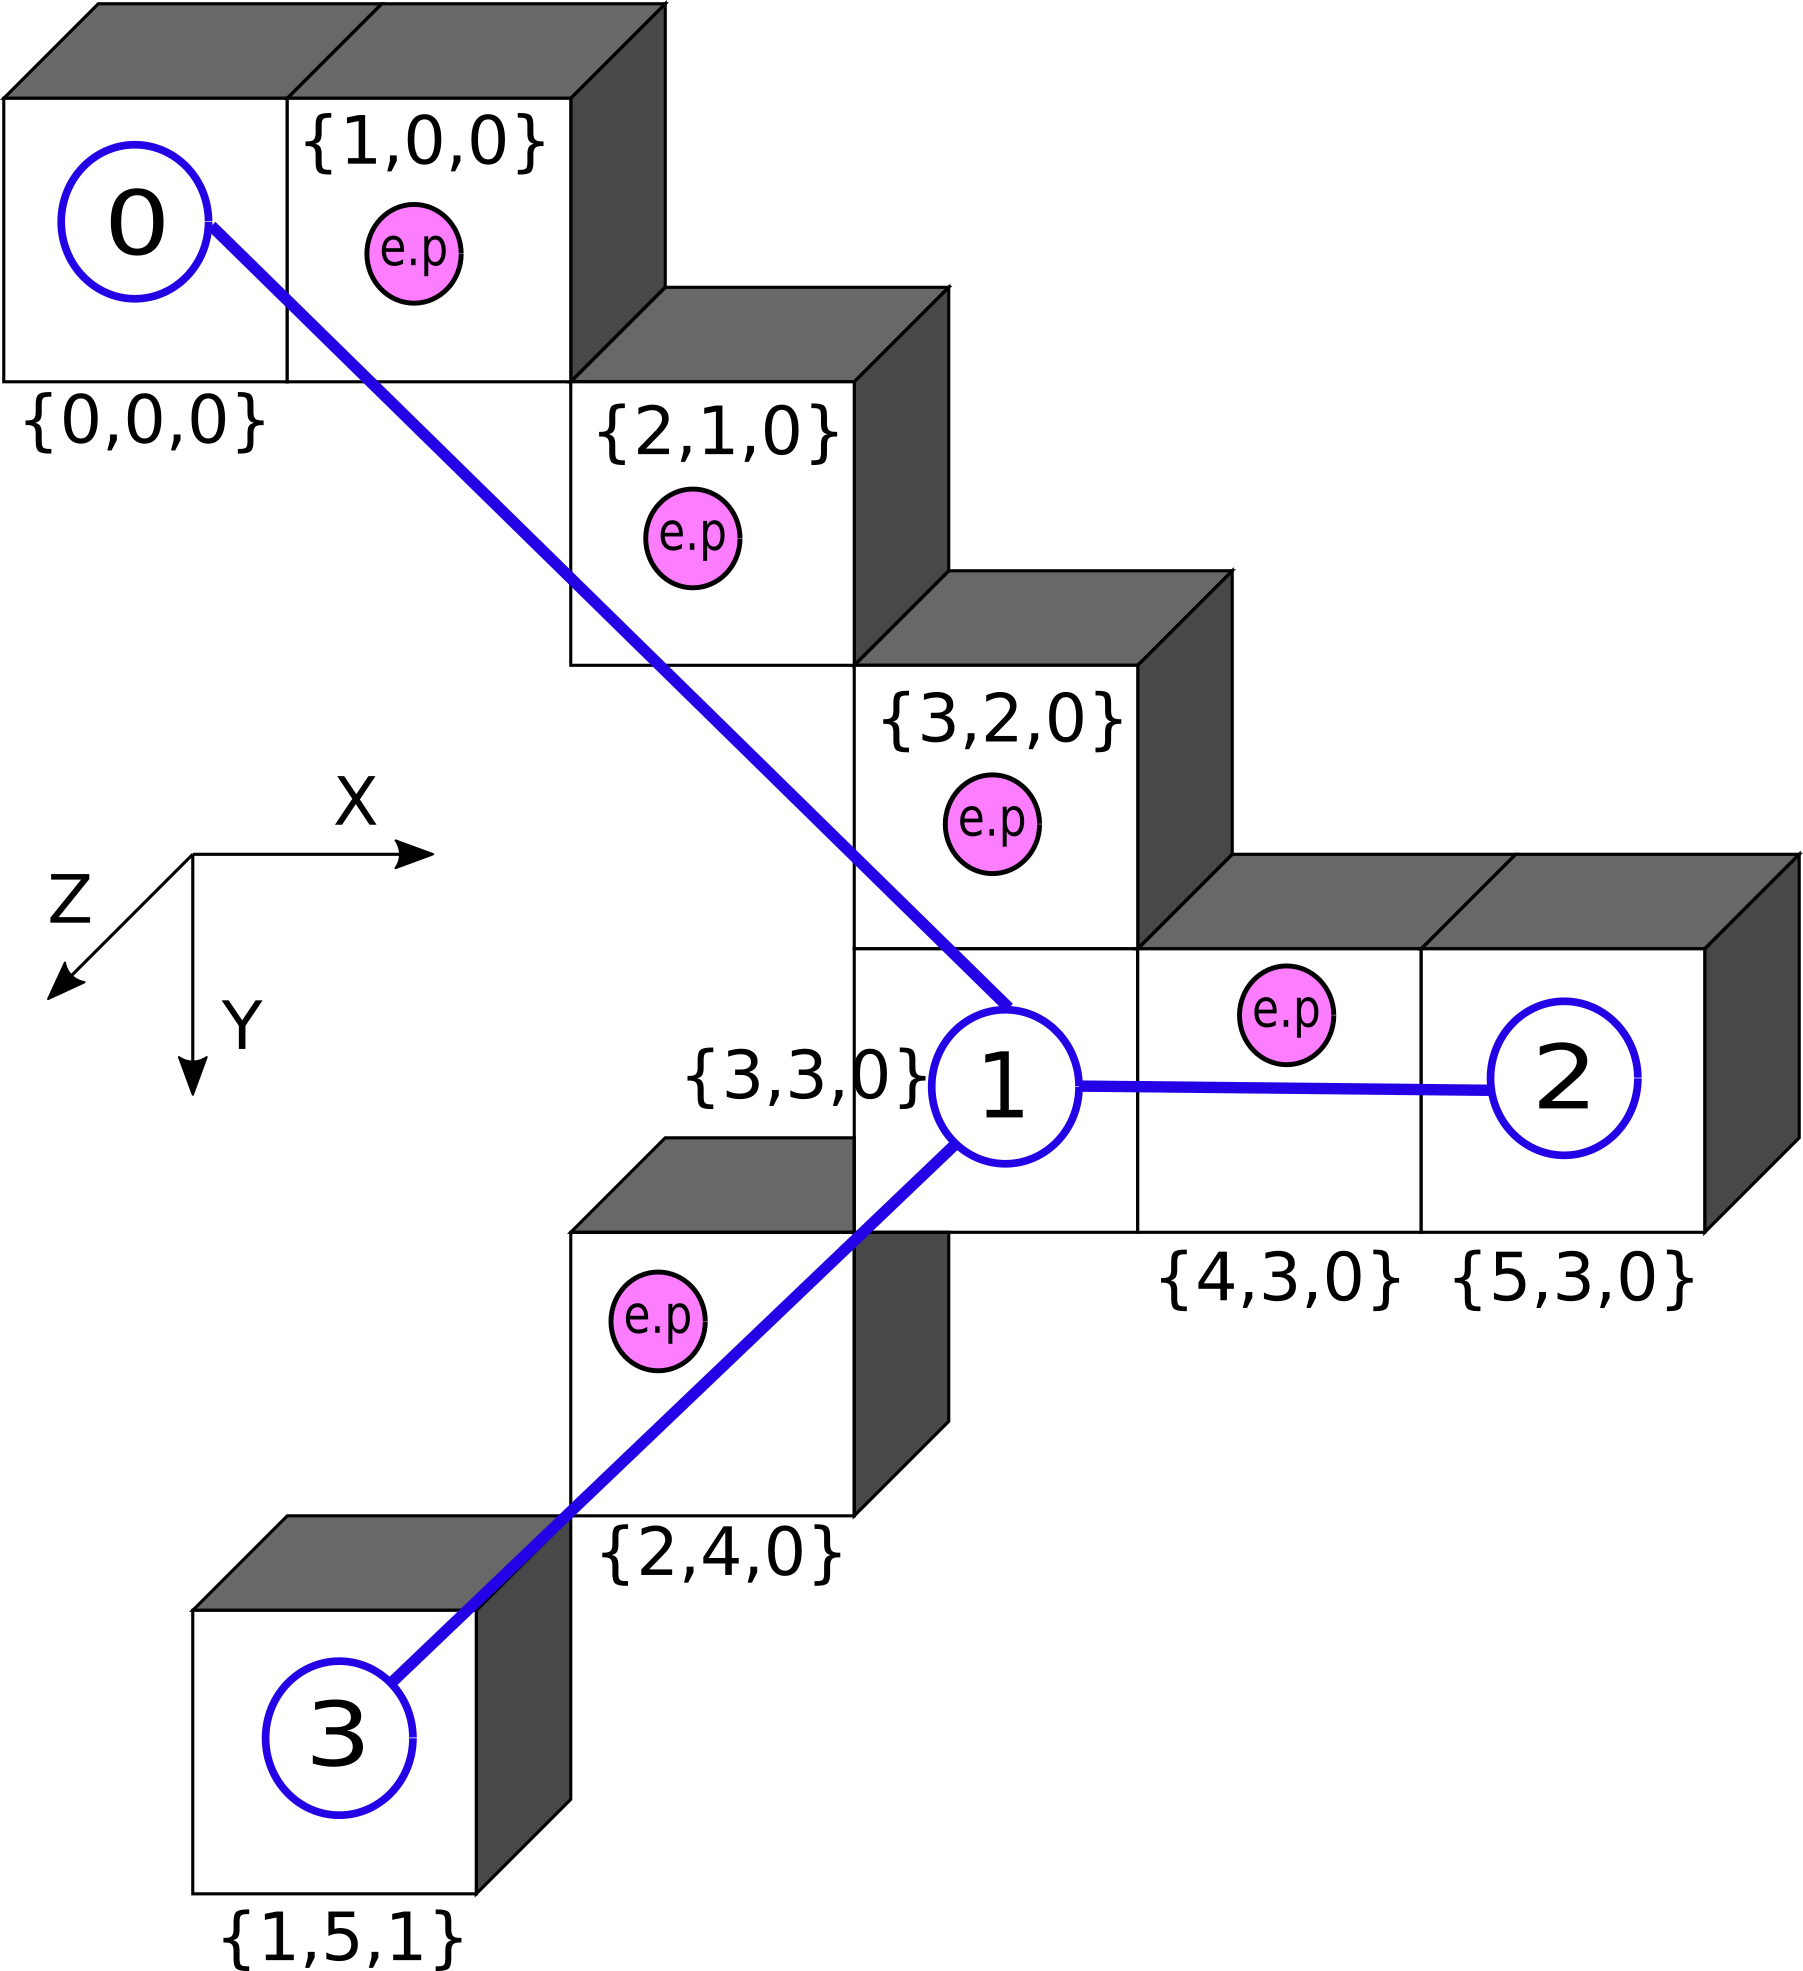
\includegraphics[width=0.6\textwidth]{Figures/chapter-image/spatial_graph_intro1.png}%
  \caption{\gls{Spatial Graph} extracted from a set of voxels. The numbers represent each node id.}
    \label{fig:spatial_graph_intro_1}
  \end{subfigure}%
  \begin{subfigure}{0.5\textwidth}
    \centering
    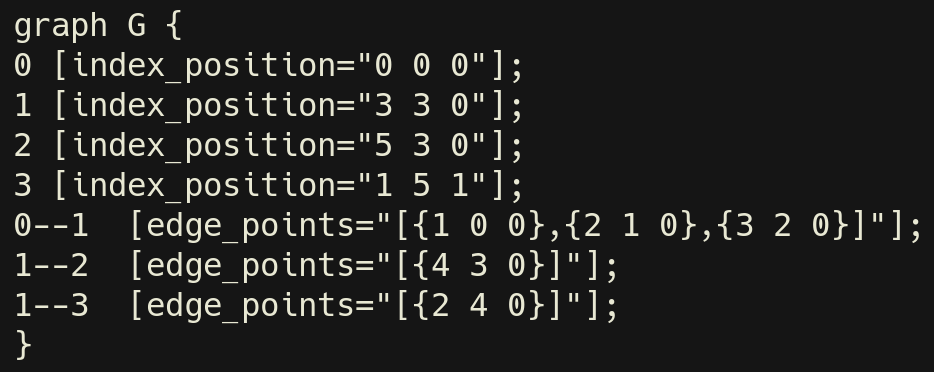
\includegraphics[width=0.9\textwidth]{Figures/chapter-image/spatial_graph_intro2.png}%
    \caption{Adjacency list representing the graph with labels containing the position of nodes and edges points.}
    \label{fig:spatial_graph_intro_2}
  \end{subfigure}%
    \caption{\gls{Spatial Graph} }
  \label{fig:spatial_graph_intro}
\end{figure}

This representation fully contain all the information needed to describe a network structure, as described elsewhere \cite{palmer_constitutive_2008}:
\begin{enumerate}[topsep=0pt]
  \item Distribution in the distance between nodes, i.e. end-to-end distances.
  \item Distribution in the fully extended length of edges, i.e. contour lengths.
  \item Network connectivity, i.e. degree of a node representing the number of other nodes connected to it.
  \item Orientation distribution. i.e. angles and director cosines of angles between adjacent edges.
\end{enumerate}

To accomplish a reliable extraction of the spatial graph from volumetric images, first we will introduce the image processing analysis used to segment the biopolymer from images, the pre-processing and denoising steps in \autoref{sec:denoising} and the binarization in \autoref{sec:segmentation}.

Secondly, we present the thinning or skeletonization
algorithm developed for creating a thin (one-pixel wide) image representation of the network in \autoref{sec:skeletonization}.

Thirdly, from the thin image, we will get the abstract representation in \autoref{sec:spatial_graph_extraction}, in form of the described \gls{Spatial Graph}.

We can compute any \gls{graph} property from our spatial graph using the tool-set of complex networks,
from degree distribution to clustering coefficient, but also the spatial information allow us to compute geometric quantities, such as distance between nodes or angle between adjacent edges.

Finally, we will compute in \autoref{sec:statistical_distributions_of_graph_properties} statistical distributions from our graph, degree, end-to-end distances, contour lengths and director cosines, that capture, in an analytical form, the network architecture.

\begin{enumerate}
  \item \hyperref[sec:denoising]{Denoising}

    \begin{itemize}
      \item Wavelet phase analysis
      \item Total Variation
    \end{itemize}

  \item \hyperref[sec:segmentation]{Segmentation}

    \begin{itemize}
      \item \hyperref[sub:binarization]{Binarization}
      \item \hyperref[sub:hole_filling]{Hole Filling}
    \end{itemize}

  \item \hyperref[sec:skeletonization]{Thinning / Skeletonization}

    \begin{itemize}
      \item \hyperref[sub:critical_kernels_framework]{Critical Kernels Framework}
    \end{itemize}

  \item \hyperref[sec:spatial_graph_extraction]{Spatial Graph Extraction}
\end{enumerate}

% Second, we will explain the two
% methods that we have tested, FIRE and Avizo. At the same time, using confocal
% images of actin networks obtained from our lab,  we will extract statistical
% distributions of some properties of the network using both algorithms. Finally,
% we will compare the results from both algorithms, and comment about future
% directions and improvements.

\subsection{Notation}%
\label{sub:notation}

 We define the \textbf{pixel}, \textbf{pixel position}, or \textbf{pixel index}  in the stack of images as:
 $\vect{p}\equiv(x,y,z)\, \epsilon \,V$, where
 $x\eps{}[0,X - 1]$, $y\eps{}[0,Y - 1]$, $z\eps{}[0,Z - 1]$ are the integer coordinates and
 $V\subset \mathbb{I}^3$ is the volume of the stack of images $V=\{X\times
 Y\times Z\}$.
 With $Z$ the number of images in the stack, and $X,Y$ the size of the $2D$ images.

 \textbf{Pixel value} or \textbf{pixel intensity} refer to the value of the pixel in the corresponding
 image.
 The value could be an integer, a boolean, or a real number, depending on if we are
 talking about a gray-scale image, a binarized image or a distance map.
 The original \textbf{gray-scale image} $I$ is defined as:
 $I(\vect{p}):V \longrightarrow G$ where
 $G$ is a set of integers representing the gray-scale.
 $G=\{0,1,\ldots,G_M\}\subset\mathbb{I}$ where $0$ represents black, $G_M$
pure white, and the others correspond to different gray-scale values. $G_M=255$
in $8$ bits images, and $G_M=2^{16} - 1 = 65535$ in higher quality images of $16$ bits.

The \textbf{binarized image} B is defined as the map:
$$f_B: I \longrightarrow B_T \,\,|$$ 
\begin{equation}
 B_T(\vect{p})=
   \begin{cases} 
     1               & \mbox{if } I(\vect{p}) > T   \\
     0               & \mbox{if } I(\vect{p}) < T
   \end{cases}
   \label{eq:bin}
\end{equation}
Where $T\eps{}G$ is the threshold value of the binarization. The threshold can also be expressed as
a normalized intensity value $T_P \eps{}[0,1]\subset \mathbb{R}$. If
$I_{max}\eps{}G$ is the max value of $I$, then the threshold  is
$T=round(T_P \cdot I_{max})$  where the round function converts a real number
into the nearest integer. The binary threshold can also be characterized with a percentage of the
brightest gray-scale value involving
cumulative histograms of $I$.

\section{Denoising}%
\label{sec:denoising}

Pre-processing the image to remove spurious noise is fundamental to obtain a good segmentation of our network in the next step.

% Add/Show wavelet denoising, and TotalVariation (proxTV)
We use the wavelet tools developed in ~\autoref{Chapter-Wavelets} to perform a phase analysis \cite{held_steerable_2010} in the image. This will equalize local brightness differences, and homogenize intensity values of foreground objects. Then we perform an anisotropic denoising, that avoids blurring information in edges of objects.

We also apply total variation \cite{barbero_fast_2011, barbero_modular_2014} methods to our 3D images, showing effective denoising and maintaining sharp transitions between edges of objects and background.

% Figure with results, one for each process.
\begin{figure}[!htb]
  \centering
  \begin{subfigure}{0.5\textwidth}
    \centering
    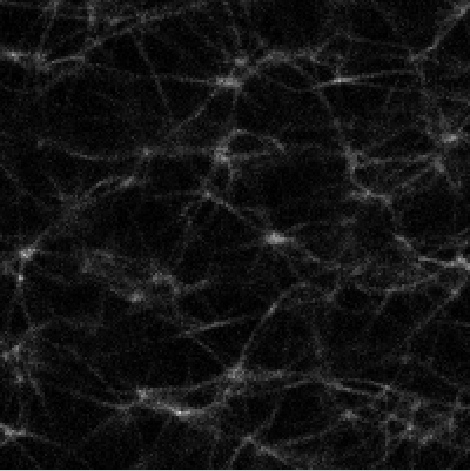
\includegraphics[width=0.9\textwidth]{Figures/chapter-image/binary/fig_bin_original.png}%
    \caption{Wavelet based}
    \label{subfig:denoise_wavelet}
  \end{subfigure}%
  \begin{subfigure}{0.5\textwidth}
    \centering
    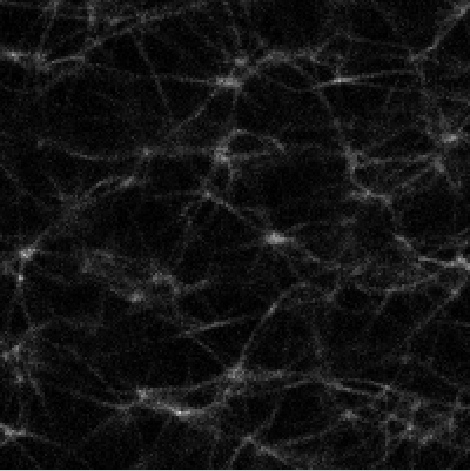
\includegraphics[width=0.9\textwidth]{Figures/chapter-image/binary/fig_bin_original.png}%
    \caption{Total Variation}
    \label{subfig:denoise_tv}
  \end{subfigure}%
  \caption{Pre-processing the image: denoising with wavelets and total variation methods.}
  \label{fig:denoise}
\end{figure}


\section{Segmentation}
\label{sec:segmentation}

Segmentation refers to the extraction of the objects of interest from an image, discarding the rest of information. When the image is composed by many different objects, with different shapes and pixel
intensities, complex approaches must be taken to reliably extract the objects of interest.
For example in biology the segmentation might want to extract only cells of certain type from an
image with many other actors.

In our case, our images are only composed by biopolymers, so our segmentation is easier, it reduces
to a binarization task: separate background and noise from the biopolymer objects.

Easier doesn't mean easy though, grouping all the information into two clusters is inherently hard.
We look for an intensity value that acts as a threshold for the two groups.
If the intensity along the image is not equalized, it might happen that objects with absolute lower intensity are lost.
This is the reason we will use a local approach, using a region growing algorithm, where we first select seeds in the middle of our object of interest, and the algorithm will grow those seeds to fill the whole region of interest, based on intensity differences between neighbor pixels and the seeds.

Any binarization filter is seriously affected by noise present in the images. That is why the pre-processing and denoising step is fundamental to get a reliable result from this process.

\subsection{Binarization}
\label{sub:binarization}
The gray levels of pixels belonging to an object are substantially
different from the gray levels of the background. Thresholding is a way to
separate objects from the background.

\citet{sezgin_survey_2004} is a good review about the subject. The output of the
thresholding process is a binary image, whose one state will indicate the
foreground objects, while the complementary state will correspond to the
background.\\
\begin{equation}
P'_i=
   \begin{cases} 
     1               & \mbox{if } I(\vect{p}) > T   \\
     0               & \mbox{if } I(\vect{p}) < T
   \end{cases}
   \label{eq:bin2}
\end{equation}
Where $P'_i\,\epsilon \, \{0{,} 1\}$ is the binarized output pixel , $P_i\,
\epsilon \,[0{,}255]$ is the gray-scale input pixel, and $T\,
\epsilon \,[0{,}255]$ is the threshold value. Note that the max value in the
grey scale could vary depending on the number of bits of the image. $255$ is
the max value for $8$ bits images;
in the case of high quality images of $16$ bits, the max value will rise to
$2^{16} - 1 = 65535$. In both cases the max value corresponds to pure white and
$0$ to black.

\begin{figure}[!htb]
\begin{subfigure}{0.5\textwidth}
  \centering
  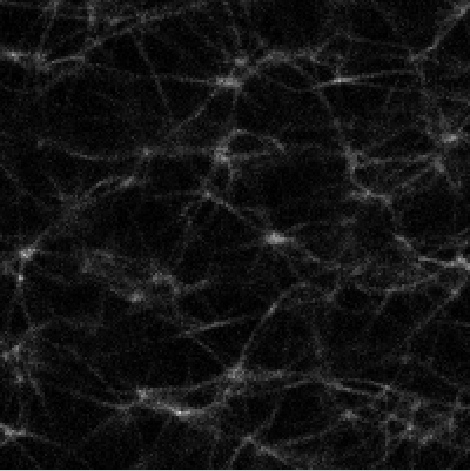
\includegraphics[width=0.9\textwidth]{Figures/chapter-image/binary/fig_bin_original.png}%
  \caption{Input Image - Original}
  \label{binoriginal}
\end{subfigure}%
\begin{minipage}{0.5\textwidth}
  \centering
  \begin{subfigure}{0.5\textwidth}
    \centering
    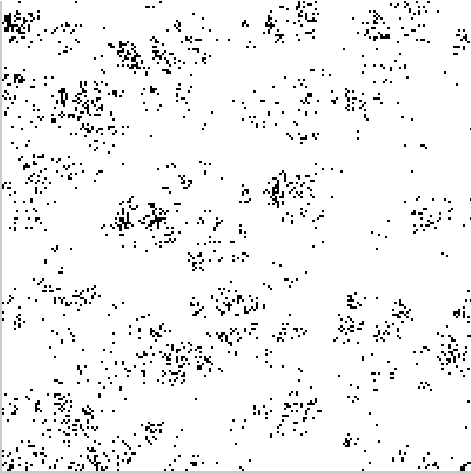
\includegraphics[width=0.9\textwidth]{Figures/chapter-image/binary/fig_bin_01.png}%
    \caption{$T_P$=0.01}
    \label{bin001}
  \end{subfigure}%
  \begin{subfigure}{0.5\textwidth}
    \centering
    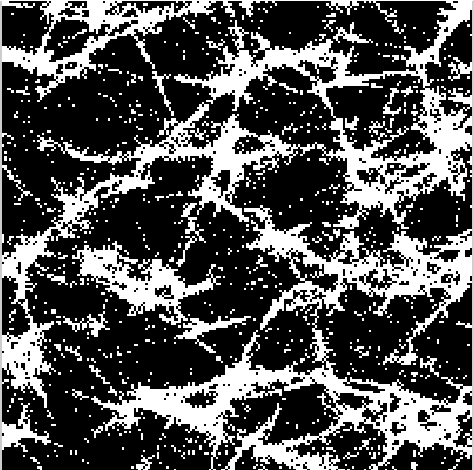
\includegraphics[width=0.9\textwidth]{Figures/chapter-image/binary/fig_bin_08.png}
    \caption{$T_P$=0.08}
    \label{bin008}
  \end{subfigure}

  \begin{subfigure}{0.5\textwidth}
    \centering
    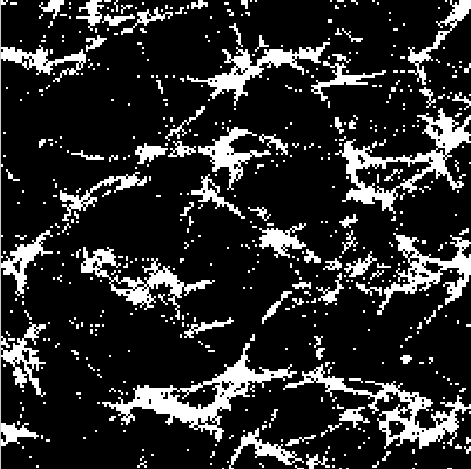
\includegraphics[width=0.9\textwidth]{Figures/chapter-image/binary/fig_bin_01176Otsu.png}%
    \caption{$T_P$=0.1176}
    \label{binotsu}
  \end{subfigure}%
  \begin{subfigure}{0.5\textwidth}
    \centering
    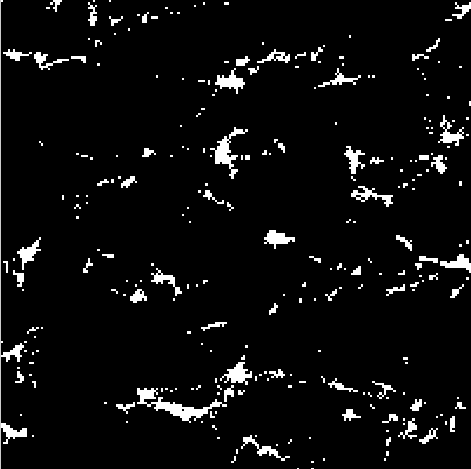
\includegraphics[width=0.9\textwidth]{Figures/chapter-image/binary/fig_bin_20.png}%
    \label{bin020}
    \caption{$T_P$=0.20}
  \end{subfigure}%
\end{minipage}

\caption[Different threshold values on networks]{Different threshold values in
Actin network.
$T_P$ is a normalized threshold value, if $G_{max}$ is the brightest pixel, then
$T=T_P\cdot P_{max}$. According to eq \ref{eq:bin}, any pixel which value is greater than T transforms to $1$
(white) after the binary filter.
At low values of threshold (case \subref{bin001}), we have blurred networks, but
at high values (case \subref{bin020}), some connectivity information is lost.
The case \subref{binotsu} corresponds to the threshold calculated by the Otsu's
method } 
\label{fig:binary}
\end{figure}

There is a lot of research in thresholding. One of the most famous binary
filters is Otsu's method, which minimizes the weighted sum of within-class variances of the
foreground and background pixels to establish an optimum threshold
\citep{sezgin_survey_2004}. This method belongs to the clustering-based methods
of thresholding. Further classification of thresholding is based on:
\begin{itemize}
  \item \textbf{Histogram shape.} Peaks, valleys and curvatures of the smoothed
  gray-level histogram are analyzed. \emph{Peak-and-valley}
  \item \textbf{Clustering.} The gray levels are clustered in two parts, one
  corresponding to the background and the other to the foreground. This method
  analyses separately each cluster. \emph{Otsu, Minimum error, fuzzy}.
  \item \textbf{Entropy.} Exploits the entropy of the distribution of the gray
  levels in the image. Maximization of entropy is indicative of high information transfer.
  Low cross-entropy between input gray level and output binary means
  preservation of information. \citet{pal_automatic_1983}
  were the first to use Shannon entropy in image analysis.
 \citep{pal_image_1988}
  \item \textbf{Object attribute.} Select the threshold based on some attribute
  quality between the original and binarized image. \emph{Edge matching, connectivity,
  shape compactness}.
  \item \textbf{Spatial methods}. This class not only uses the gray
  distribution, also studies the dependency of pixels in a neighborhood, for example, correlation
functions or co-occurrence probabilities.
  \item \textbf{Local adaptive methods.} A threshold is calculated at each
  pixel, which depend on some local statistics, like \emph{variance}.
  \item \textbf{Region growing.} The binarization starts from seed pixels placed in the interior
    of objects wanted to be segmented. These algorithms study the neighborhood of these seeds and under some criteria, for example intensity difference, it adds the neighbor pixel to the foreground region. The process is repeated until no new pixel is added.
\end{itemize}

For our purposes, the binarization threshold will have an impact obtaining the
network. If the threshold is too high, long fibers will break in short,
unconnected pieces. If the threshold is too low, fibers that are clearly
separated, will become blurred together.

In Fig.\ref{fig:binary}
we compare the geometry of a small area of an actin network after
applying different binary thresholds. The stack of images of
networks used here was obtained in our group by Dr. Allan
Raudsepp using confocal microscopy on actin.

\subsubsection{Region Growing Segmentation}%
\label{subsub:region_growing_segmentation}

The risk of region growing algorithms is to plant a seed outside our foreground objects, we have found ideal to plant the seeds with a normalized threshold $T_p$, so we don't have to fine tune the lower threshold too much. The results are quite resilient against small changes of these parameters, where a pure thresholding approach will suffer a lot of variation and be prone to noise artifacts.

Using \href{https://itk.org/Doxygen/html/classitk_1_1ConnectedThresholdImageFilter.html}{itk::ConnectedThresholdImageFilter} with the script:
\href{https://github.com/phcerdan/ITKfilters/blob/master/scripts-cpp/regionGrowingSegmentation.cxx}{regionGrowingSegmentation.cxx}

\noindent\textbf{Parameters:}

\begin{itemize}[topsep=0pt]
  \item \textbf{Lower threshold} and \textbf{upper threshold: } The region won't grow into pixels outside these limits. Combined with a conservative $T_p$ for initial seeds the results does not change with small variation of these parameters.
  \item \textbf{Normalized Threshold $T_p$ for initial seeds: } Create initial seeds based on a normalized binary threshold. This should take a conservative low value, the region will grow anyway from these seeds to fill the object.
\end{itemize}

\subsection{Hole Filling}%
\label{sub:hole_filling}

Due to noise, tiny holes might still be created in the binarization process. These holes (areas of OFF pixels surrounded by ON pixels) have an important effect in the following skeletonization step because they change the topology of the object and the network we want to extract. To solve it, we aggressively fill these small holes with an iterative hole filling algorithm.


Using \href{https://itk.org/Doxygen/html/classitk_1_1VotingBinaryIterativeHoleFillingImageFilter.html}{itk::VotingBinaryIterativeHoleFillingImageFilter} with the script:
\href{https://github.com/phcerdan/ITKfilters/blob/master/scripts-python/binary_denoise_3d_fillholes_iterative.py}{binary denoise 3D fillholes}

\noindent\textbf{Parameters:}

\begin{itemize}[topsep=0pt]
  \item \textbf{Majority: } Number of ON pixels in the neighborhood of an OFF pixel, to switch it into ON. By default, majority = 1, this means that an off pixel will be turned on if in the neighborhood (set by radius) there are at least 50\% + 1 pixels ON. If $\text{radius} = \{1,1,1\}$ neighborhood size will be $3\times3 = 9$ pixels. If 5 pixels around an OFF pixel are ON, then it will be switched.
  \item \textbf{Neighbor Radius: } Number of neighbors to check. $R = 1$ in 3D is a $3\times3\times3$ neighborhood.
  \item \textbf{Iterations: } Number of iterations before stopping, the algorithm also stop if no changes are generated after last iteration.
\end{itemize}

For our networks, we have found optimal values in:\newline
Majority = 3, Radius = 1, Iterations = $\infty$ \newline
The high value of majority and the small neighborhood only fills small holes.



\section{Skeletonization}%
\label{sec:skeletonization}

The skeleton of an object is a representation of the object, which contain both,
shape features and topological structures of the original object. It is widely
used in computer graphics, character recognition, and analysis of biomedical
images.\citep{bai_skeleton_2007,golland_fixed_2000,ge_generation_1996}. The
skeletonization is very sensitive to noise and boundary deformations, which generates redundant skeleton branches that disturb the
topology of the skeleton graph (Fig.\ref{fig:skeleton-fixedtopo}(b)).

To overcome this instability, the methods used are based on skeleton pruning,
i.e. eliminating the spurious branches. What are then the desirable properties
of a skeletonization process?
\begin{enumerate*}[label=\textbf{\alph*)}]
  \item Preserve the topology of the original object, i.e. it has the same tails
  and/or holes.
  \item Accurate position.
  \item Contain the centers of maximal disks, which can be used for the
  reconstruction of the original object
  \item Stable under small deformation and noise.
\end{enumerate*}

\begin{figure}[!htb]
  \centering
  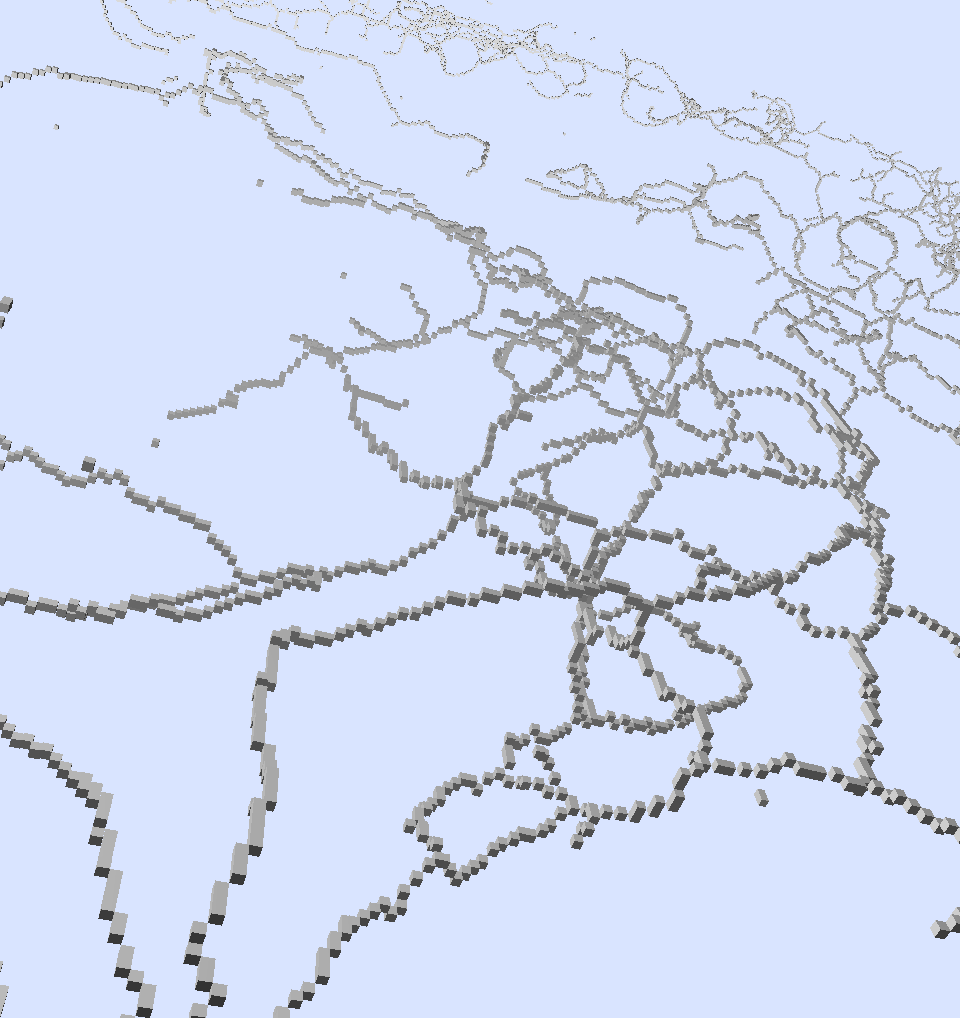
\includegraphics[width=0.8\textwidth]{Figures/chapter-image/skeleton_3D_viewer.png}%
  \caption{Thin image of a pectin network after skeletonization (see \autoref{sub:Pectin}) visualized with a 3D Viewer.}
  \label{fig:thin_3Dviewer}
\end{figure}

The most important skeletonization algorithms
can broadly be classified into three types:

\begin{enumerate}
  \item Based on Voronoi diagrams \citep{ogniewicz_hierarchic_1995}.
    These methods search the locus of centers of the maximal disks
    contained in the contour of the object. The skeleton can be
    extracted with accurate position and topology, but the time
    of computation is usually prohibitive, and the complicated skeleton needs to be
    pruned.
  \item Based on detecting ridges
    in the distance map from the boundary points. The
    position is accurate, but does not guarantee correct topology
    \citep{ge_generation_1996}. It is widely used because the computation
    affordability. The two methods analyzed from literature are based on
    this kind of skeletonization.
  \item Based on the critical kernels framework, where the removing of
    voxels (pixels in 3D) is ensured to maintain the original topology of the object \cite{couprie_asymmetric_2016}.
    I contributed with this framework to DGtal \url{https://github.com/DGtal-team/DGtal} \cite{david_coeurjolly_dgtal-team/dgtal:_2018}, an open-source digital topology
    library in c++.
    The work was reviewed, accepted and merged in the library since version 0.9.4 (see~\ref{sub:contribution_dgtal} for more information).
\end{enumerate}

\subsection{Critical Kernels Framework}%
\label{sub:critical_kernels_framework}

I refer the interested reader to the original work of Bertrand and Couprie about Critical Kernels \cite{bertrand_parallel_2017}. Here I will introduce a short summary of the framework, and options for the script used in this work. This summary was contributed to the \href{https://dgtal.org/doc/nightly/moduleVoxelComplex.html}{documentation of DGtal library} by the author.

\begin{itemize}[topsep=0pt]
  \item \textbf{Isthmus: } ``Intuitively a voxel x of an object X is said to be a 1-isthmus (resp. a 2-isthmus)
    if the neighborhood of x corresponds -up to a thinning- to the one of a point belonging to a curve (resp. a surface)."
  \item \textbf{Reducible: } We say that the complex X is reducible only if it is possible to reduce it (with thinning) to a single voxel.
  \item \textbf{d-cell: }
    A d-cell where $ d \in \{0,1,2,3\} $ is a pointel for $d = 0$, a linel for $d = 1$, a surfel for
    $d = 2$, or a spel for $d = 3$.

    For example, a voxel contains 1 spel, 6 surfels, 12 linels, and 8 pointels. And the intersection of two neighbor voxels sharing a face contains 1 surfel, 4 linels and 4 pointels.
  \item \textbf{Clique: }
    Let $ d \in \{0,1,2,3\} $ and let $ C \in V^3 $ with $V^3$ being the collection of all
    voxel complexes (a finite set composed solely of voxels).
    We say that C is a d-clique if the intersection of all voxels of C is a d-cell.

    Any complex C made of a single voxel is a 3-clique. Furthermore, any voxel of a complex
    constitutes a 3-clique that is \textbf{essential} for X. Essential is the minimal clique for X.
  \item \textbf{K-neighborhood (of voxel S): }
    $K(S)$ is the set of all voxels adjacent to S. And $K^*(S) = K \setminus  S$.
  \item \textbf{Regular Clique: }
    We say that the clique C is \textbf{regular} for X if $K^*(C) \cap X $ is \textit{reducible} to a
    single voxel.
  \item \textbf{Critical Kernel: }
    We say that C is \textbf{critical} for X if C is not regular.
    Note that if C is a single voxel x, then C is regular for X, only if x is simple for X.
\end{itemize}

Removing simple voxels in parallel is known to change its topology, but using \textit{critical kernels} it is ensured to keep the same topology and homotopy type after thinning.

\begin{theorem}
  The complex Y is a thinning of X if any clique that is \textbf{critical} for X,
  contains at least one voxel of Y.
\end{theorem}

The details of the algorithm can be summarized in the implementation of four masks
$K_0$, $K_1$, $K_2$, $ K_3$, that given a d-cell (pointel, linel, surfel, spel) return a d-clique and a boolean flag with its criticality. Where $K_3$ corresponds to the well-known simplicity check of a voxel. We then apply an iterative thinning algorithm shown in \autoref{fig:algo_persistence}.

\begin{figure}[!htb]
  \centering
  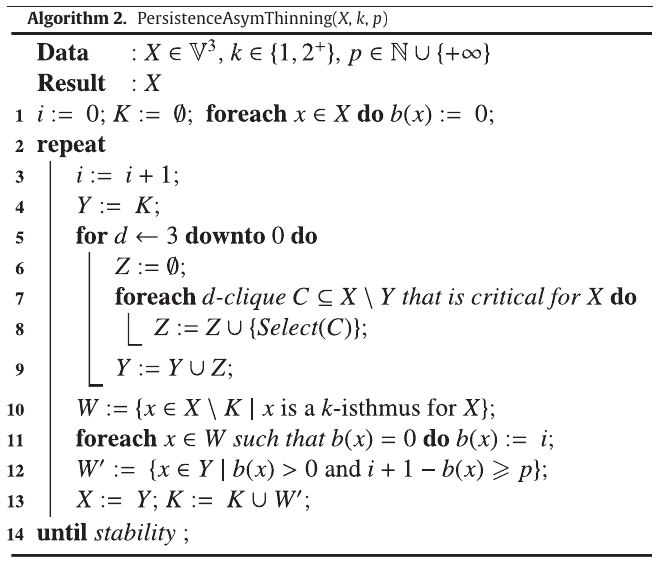
\includegraphics[width=0.8\linewidth]{Figures/chapter-image/dgtal/voxelComplexAlgoPersistence.png}
  \caption{Asymmetric thinning algorithm with persistence, from Ref.~\cite{couprie_asymmetric_2016}}
  \label{fig:algo_persistence}
\end{figure}

Based on this framework we also implement the concept of persistence of a voxel in the thinning \cite{couprie_asymmetric_2016}. The motivation is to automatically prune those branches that do not belong to a robust skeleton.

Let $i$ be the generation (see \autoref{fig:algo_persistence}) at which a voxel $x$ becomes an isthmus for the first time, we name it \textit{birth date} $b(x) = i$ of the voxel. In a later generation $j$ of the thinning process, the voxel might become deletable, we call it \textit{death date} $d(x) = j$.
The definition of \textit{persistence} of a voxel is the difference between death and birth date, $p(x) = d(x) - b(x)$.
We can choose to only keep isthmuses that have a persistence greater than a selected threshold. This persistence can be interpreted as a relative measure of the elongation of an object. With the persistence parameter, the user decides how much the elongation of an object must exceed its width to be preserved. This effectively prune short and insignificant branches.

\begin{figure}[!htb]
  \centering
  \begin{subfigure}{0.333\textwidth}
    \centering
    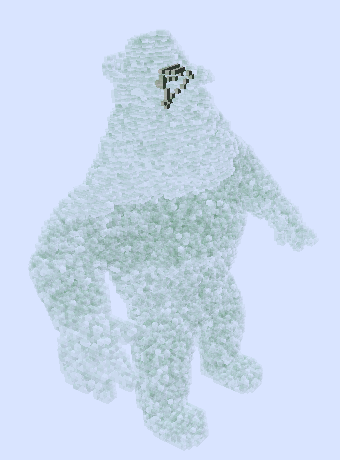
\includegraphics[width=0.95\textwidth]{Figures/chapter-image/dgtal/voxelComplexAlUltiP0.png}%
    \caption{}
    \label{subfig:thin_al_ulti}
  \end{subfigure}%
  \begin{subfigure}{0.333\textwidth}
    \centering
    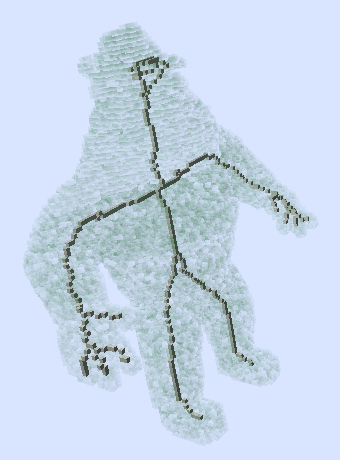
\includegraphics[width=0.95\textwidth]{Figures/chapter-image/dgtal/voxelComplexAl1IsthtmusP0.png}%
    \caption{}
    \label{subfig:thin_al_p0}
  \end{subfigure}%
  \begin{subfigure}{0.333\textwidth}
    \centering
    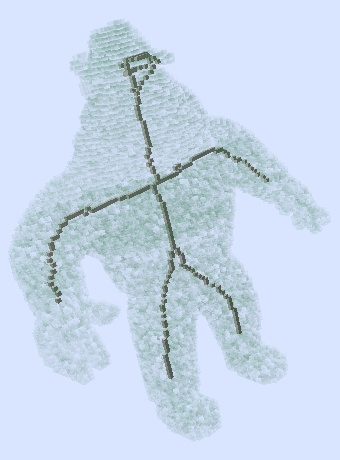
\includegraphics[width=0.95\textwidth]{Figures/chapter-image/dgtal/voxelComplexAl1IsthtmusP10.png}%
    \caption{}
    \label{subfig:thin_al_p10}
  \end{subfigure}
  \caption{Asymmetric thinning of a volume with different parameters. (\subref{subfig:thin_al_ulti}): Ultimate skeleton, only voxels that conserve topology are kept. (\subref{subfig:thin_al_p0}): keeps 1-isthmus as part of the skeleton. (\subref{subfig:thin_al_p10}): 1-isthmus with persistence parameter $p = 10$}
  \label{fig:thin_al}
\end{figure}

The implementation also allows unlimited flexibility, thanks to a functional style, to choose the \textit{Select} and \textit{Skel} function for any purpose.

The \textit{Select} function chooses a voxel from a given pool. This is necessary given the parallel or asymmetric nature of the algorithm. The options are:

\begin{itemize}[topsep=0pt]
  \item \textbf{selectRandom: } Given a set of voxels (a clique), chooses one at random.
  \item \textbf{selectFirst: } Select the first voxel in lexicographical order.
  \item \textbf{selectMaxValue: } Select a voxel with the max value of another user-defined function. We will use this wrap to use a distance map (See \autoref{subsub:distance_maps})
\end{itemize}

The \textit{Skel} function provides a way to keep voxels that we want preserve in the final skeleton.

\begin{itemize}[topsep=0pt]
  \item \textbf{skelUltimate: } Null, only preserve voxels which removal alters the topology.
   The result of the thinning in a solid object without holes and no branches is just one voxel.
  \item \textbf{skelEnd: } Preserve voxels that has only one neighbor.
  \item \textbf{OneIsthmus: } Preserve 1-isthmus voxels.
  \item \textbf{TwoIsthmus: } Preserve 2-isthmus voxels.
  \item \textbf{skelIsthmus } Preserve 1 and 2-isthmus voxels.
  \item \textbf{skelWithTable } Accepts a look-up-table (LUT) of pre-computed values of certain property for certain configuration of voxels. This is used with pre-computed LUT tables for isthmus to greatly speed up the computation. It is greatly recommended and LUT tables for 26\_6 (fully connected in 3D) topology are provided.
\end{itemize}

\begin{figure}[!htb]
\begin{center}
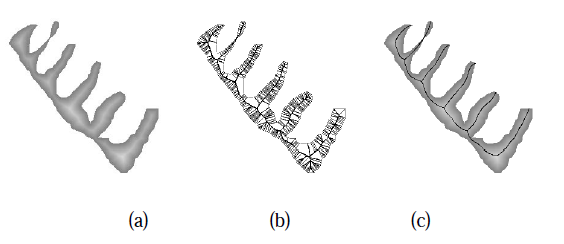
\includegraphics[width=0.8\textwidth]{Figures/chapter-image/skeleton-fixedtopo_letters.png}%
\caption[Skeletonization]{Skeletonization process. (a) Distance
map. (b) Traditional skeleton with no pruning. (c) Skeleton generated using
fixed topology methods. From Ref.\citep{bai_skeleton_2007,golland_fixed_2000}}
\label{fig:skeleton-fixedtopo}
\end{center}
\end{figure}


\subsubsection{Distance maps}%
\label{subsub:distance_maps}

The distance map calculates the distance from a
white pixel to the nearest black pixel. Every white pixel in the binary image
has now a real value calculated using any selected distance function (euclidean,
quasi-euclidean,\ldots ). Distance maps can be calculated from a binary image, or to
any image with shapes that are labeled differently.
Fig.\ref{fig:distancemap} has some distance maps of actin networks.
We can see in Fig.\ref{fig:fire_LMPS} the values of a distance map, which have
been simplified from real to integers for clarity.


\begin{figure}[!htb]
\begin{minipage}{0.5\textwidth}
  \centering
  \center{\textbf{Binarization}}\\
  % \begin{minipage}{0.5\textwidth}
  \begin{subfigure}{0.5\textwidth}
    \centering
    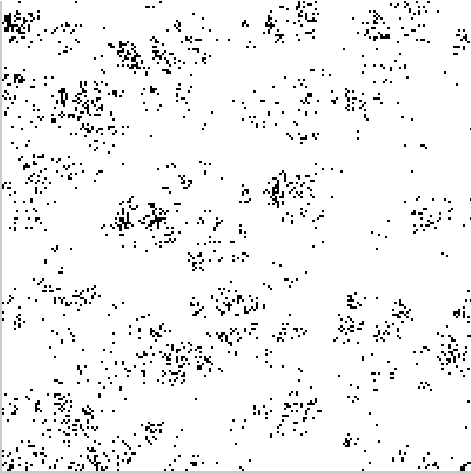
\includegraphics[width=0.9\textwidth]{Figures/chapter-image/binary/fig_bin_01.png}
    \caption{$T_P$=0.01}
  \end{subfigure}%
  \begin{subfigure}{0.5\textwidth}
    \centering
    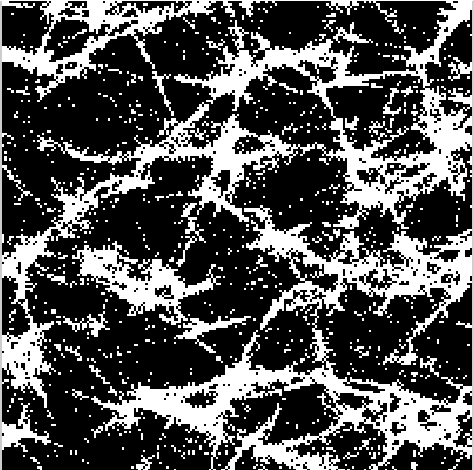
\includegraphics[width=0.9\textwidth]{Figures/chapter-image/binary/fig_bin_08.png}
    \caption{$T_P$=0.08}
  \end{subfigure}

  \begin{subfigure}{0.5\textwidth}
    \centering
    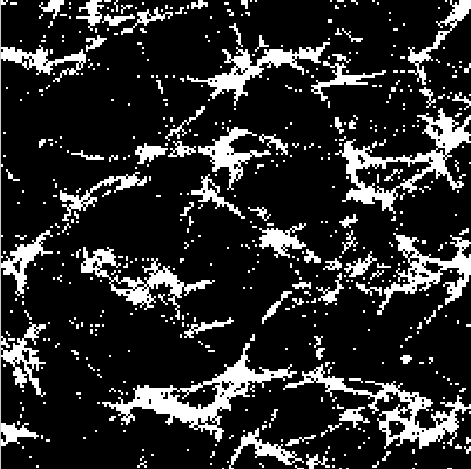
\includegraphics[width=0.9\textwidth]{Figures/chapter-image/binary/fig_bin_01176Otsu.png}
    \caption{0.1176}
  \end{subfigure}%
  % \hspace{1pt}
  \begin{subfigure}{0.5\textwidth}
    \centering
    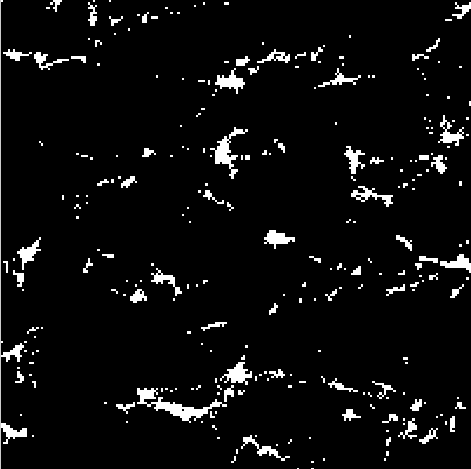
\includegraphics[width=0.9\textwidth]{Figures/chapter-image/binary/fig_bin_20.png}
    \caption{$T_P$=0.20}
  \end{subfigure}%
\end{minipage}
\begin{minipage}{0.5\textwidth}
  \centering
  \center{\textbf{Distance map}}\\
  \begin{subfigure}{0.5\textwidth}
    \centering
    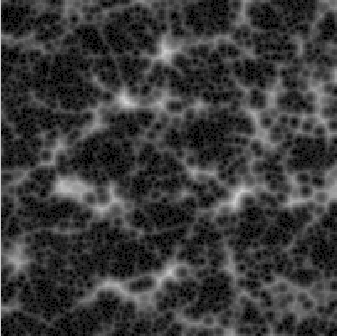
\includegraphics[width=0.9\textwidth]{Figures/chapter-image/distance/fig_dist_01.png}
    \caption{$T_P$=0.01}
  \end{subfigure}%
  \begin{subfigure}{0.5\textwidth}
    \centering
    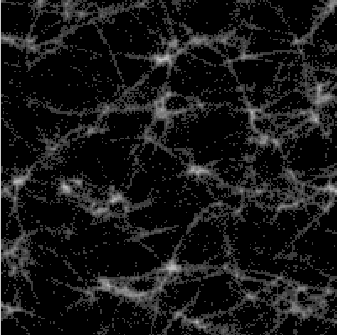
\includegraphics[width=0.9\textwidth]{Figures/chapter-image/distance/fig_dist_08.png}
    \caption{$T_P$=0.08}
  \end{subfigure}

  \begin{subfigure}{0.5\textwidth}
    \centering
    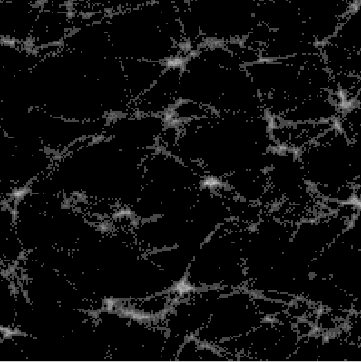
\includegraphics[width=0.9\textwidth]{Figures/chapter-image/distance/fig_dist_01176Otsu.png}
    \caption{0.1176}
    \label{distotsu}
  \end{subfigure}%
  \begin{subfigure}{0.5\textwidth}
    \centering
    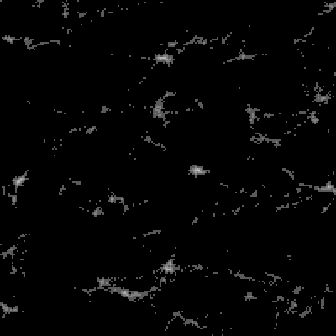
\includegraphics[width=0.9\textwidth]{Figures/chapter-image/distance/fig_dist_20.png}
    \caption{$T_P$=0.20}
    \label{dist014}
  \end{subfigure}
\end{minipage}

\caption[Distance map - Actin]{ Distance maps calculated from binarized images
with different normalized thresholds $T_P$}
\label{fig:distancemap}
\end{figure}

We use a distance map for our \textit{Select} skeletonization function, to first select the voxels which have max value in the distance map. This traduces to select the voxels in the median axis, so it is ensured to get a centered skeleton.

\subsection{Testing other thinning algorithms}%
\label{sub:testing_other_thinning_algorithms}

\subsubsection{FIbeR Extraction -FIRE-}
\label{subsub:FIRE}

FIRE has been developed in Matlab by Andrew M. Stein
  \citep{stein_mathematical_2007} to extract collagen networks from confocal
  images. It can be downloaded, and upgrades can be uploaded in
  \url{https://github.com/uw-loci/fiber-extraction}. The method
  \citep{stein_algorithm_2008} is based on an original idea of
  \citet{wu_automated_2003}. The main upgrade is the use of multiple nucleation
  points   and the restriction that each branch extends only  in a single
  direction from a nucleation point. In \citet{wu_automated_2003}  the network has a single nucleation point at the global maximum of the distance function D.


 \begin{enumerate}[label=\textbf{\Alph*}]

 \item \textbf{Smooth filter} Smooth the image with a Gaussian filter
 \item \textbf{Binarization threshold} Keep a percentage of the brightest pixels
 \item \textbf{Distance map D} Distance map using Euclidean distance. It
 assigns a value to each pixel equal to the distance from that pixel to the nearest black value.

 \item \textbf{Nucleation points NPs} They are the
 local maxima of the distance map $D(\vect{u})$. The locality is defined by a
 box of chosen radius $s_{xbox}=5$. They are only selected if they
 exceed a tunable threshold $\theta_{nuc}=2$. A single nucleation point of
 value $4$ is denoted by the thick circle in \ref{fig:fire_LMPS}\subref{LMP1}

 \item \textbf{Extension of branches LMPs} The next step is to trace the
 branches, extending from the nucleation points. To do that FIBER finds a set of
 Local Maximum Points (LMPs) at \emph{each} nucleation point. LMPs occur where
 there is a local maximum in $D(\vect{u})$ on the surface of the box centered in the NP
 $\vect{u}$, and with radius(in pixels) the rounded up value of $D(\vect{u})$.
 See Fig. \ref{fig:fire_LMPS}\subref{LMP1}. LMPs are then extended with other
 LMPs only if the direction of extension is straight enough
 (Fig. \ref{fig:fire_LMPS}\subref{LMP2}). If there is no LMP with that
 condition, or it arrives other nucleation point, the iteration ends.
 \end{enumerate}


\begin{figure}[!htb]
  \centering
  \begin{subfigure}{0.5\textwidth}
    \centering
    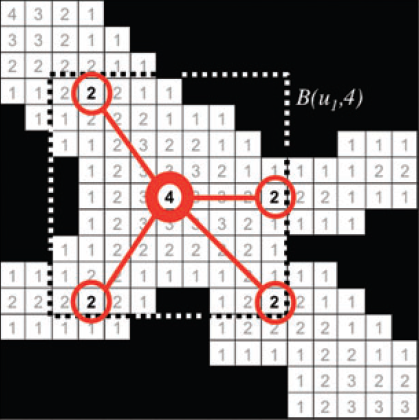
\includegraphics[width=0.8\textwidth]{Figures/chapter-image/fire/nucleation1.png}%
    \caption{Step 1}
    \label{LMP1}
  \end{subfigure}%
  \begin{subfigure}{0.5\textwidth}
    \centering
    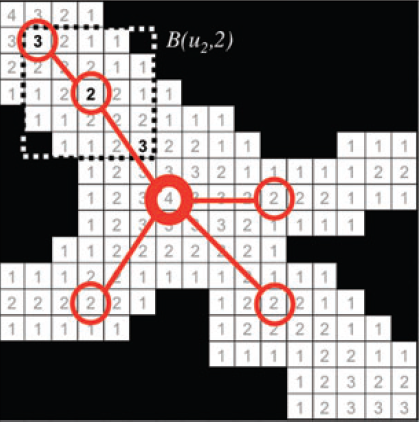
\includegraphics[width=0.8\textwidth]{Figures/chapter-image/fire/nucleation2.png}
    \caption{Step 2}
    \label{LMP2}
  \end{subfigure}
  \caption[FIRE algorithm - Find LMP]{Tracing of the ridges of the distance
    map using FIRE from Ref.\citep{stein_algorithm_2008}: \subref{LMP1} Step 1:
    Pick a nucleation point (thick circle) and find all LMPs. \subref{LMP2} Step 2:
    Pick an LMP and find the next LMP which continues in the same direction. See
  text for details.}
  \label{fig:fire_LMPS}
\end{figure}


\subsubsection{Results in FIRE}
 I have used FIRE to analyse our
 confocal stacks obtained from actin networks. For testing purposes, the images
have been cropped due to the slowness of FIRE
processing big networks. From an original image of Actin of
$V=1024\times1024\times39$, we have cropped it to $V=200\times200\times20$. 

In Fig.\ref{fig:fire_stepbystep} we can see the different steps of the FIRE
algorithm. In Fig.\ref{fig:fire_histograms} we plot the statistical distribution
of length and degree for different thresholds $T_P$. Further analysis is
required, and a bigger network for better statistics, but it seems that length
follow a log-normal distribution, and the degree, a geometrical distribution. We
will say more about distributions in chapter \ref{Chapter-Reconstruction}.

 \begin{figure}[!htb]

\begin{center}
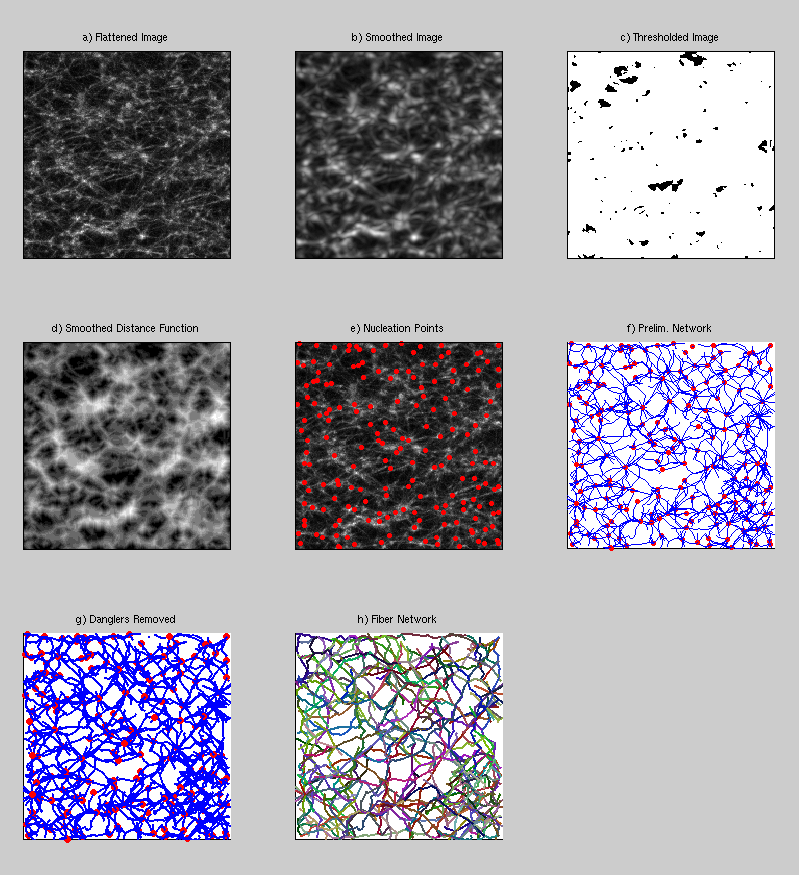
\includegraphics[width=0.9\textwidth]{Figures/chapter-image/fire/fire012.png}%

\end{center}


\caption[Fire: Step by step for $T_P=0.12$]{FIRE: step by step}
\label{fig:fire_stepbystep}
\end{figure}

\begin{figure}[!htb]
  \centering
  \begin{subfigure}{0.5\textwidth}
    \centering
    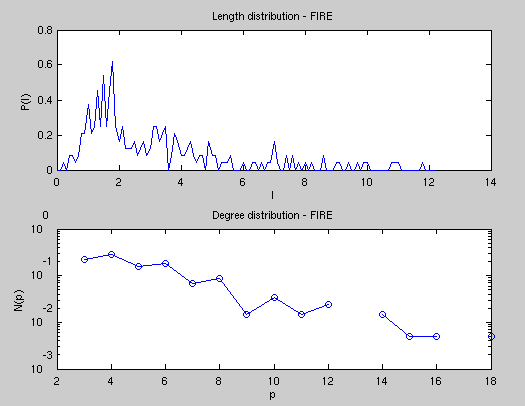
\includegraphics[width=0.95\textwidth]{Figures/chapter-image/fire/fire017histo.png}%
    \caption{$T_P=0.17$}
    \label{firehisto017}
  \end{subfigure}%
  \begin{subfigure}{0.5\textwidth}
    \centering
    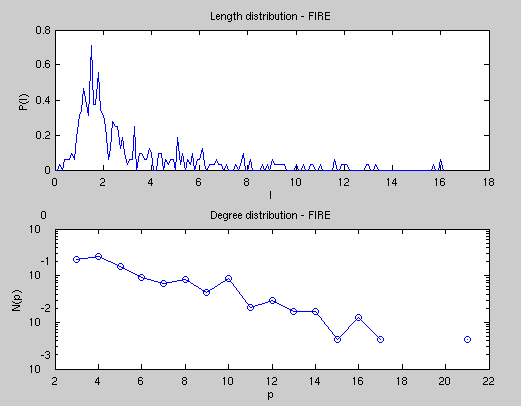
\includegraphics[width=0.95\textwidth]{Figures/chapter-image/fire/fire012histo.png}%
    \caption{$T_P=0.12$}
    \label{firehisto012}
  \end{subfigure}

  \begin{subfigure}{0.5\textwidth}
    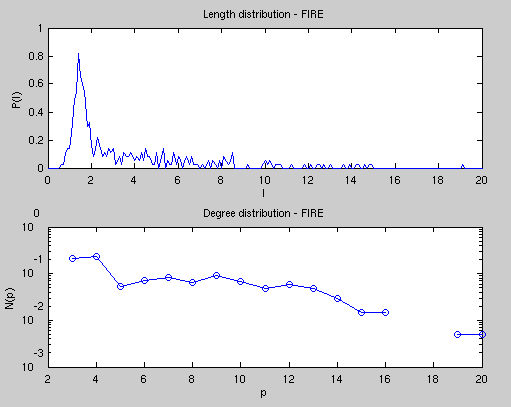
\includegraphics[width=0.95\textwidth]{Figures/chapter-image/fire/fire008histo.png}%
    \caption{$T_P=0.08$}
    \label{firehisto008}
  \end{subfigure}
\caption[Distributions of length and degree in FIRE]{Extracting statistical
distributions for different binary thresholds using FIRE from cropped
actin netwoks.}
\label{fig:fire_histograms}
\end{figure}

A useful statistical distribution is the one studying the angles between edges
that are incident to the same node. I am currently working on a way to extract
the director cosines (angles) distribution from FIRE.

\subsubsection{Avizo: XSkeleton}
 Avizo is a software commercialized by
 \href{http://www.vsg3d.com/avizo/overview}{FEI: Visualization Sciences Group}.
The access to Avizo is granted by a collaboration with Fonterra (Food company,
NZ).

\textbf{XSkeleton} is the package or module that we will use to extract the
network topology. The algorithm and the result is different to FIRE. Here
follows a description step by step:
\begin{enumerate}[label=\textbf{\Alph*}]
 \item\textbf{Smooth filter} Smooth the image with a Gaussian filter
 \item\textbf{Binarization threshold} Multi-threshold module. This threshold is
 not based in percentage of the brightest pixel. It is a classical threshold turning
 to pure white $255$ or logical $1$ all pixels with a value greatest than the
 threshold value, and black $0$ all the pixels below that value.
 \item\textbf{Distance map} Distance map using Euclidean distance. It assigns a
 value to each pixel equal to the distance from that pixel to the nearest black value. 
 \item\textbf{Thinner module} This is the \textbf{skeletonization} step. The
 module takes as input a label-field to be thinned and a distance map scalar field. It removes voxel by voxel from the segmented
 object until only a string of connected voxels remains.
 The thinning algorithm automatically detects dead end branches of skeleton
 spatial graphs. A parameter is used to distinguish them from noise on the
 interface  of the considered regions to avoid spurious branches.  Its default
 value is 5, i.e. the branches with a dead end which length is lower  than 5
 voxels are automatically considered as noise and removed.  Setting this to 10,
 which is a rather large value, leads to only a few branches remaining in the
 skeleton.  The drawback is that you also might miss real endpoints.
 
\item\textbf{Trace lines module} Converts an image that contains lines
represented by voxels into a spatial graph object.

 \end{enumerate}

\begin{figure}[!htb]

% \begin{minipage}{0.5\textwidth}
 
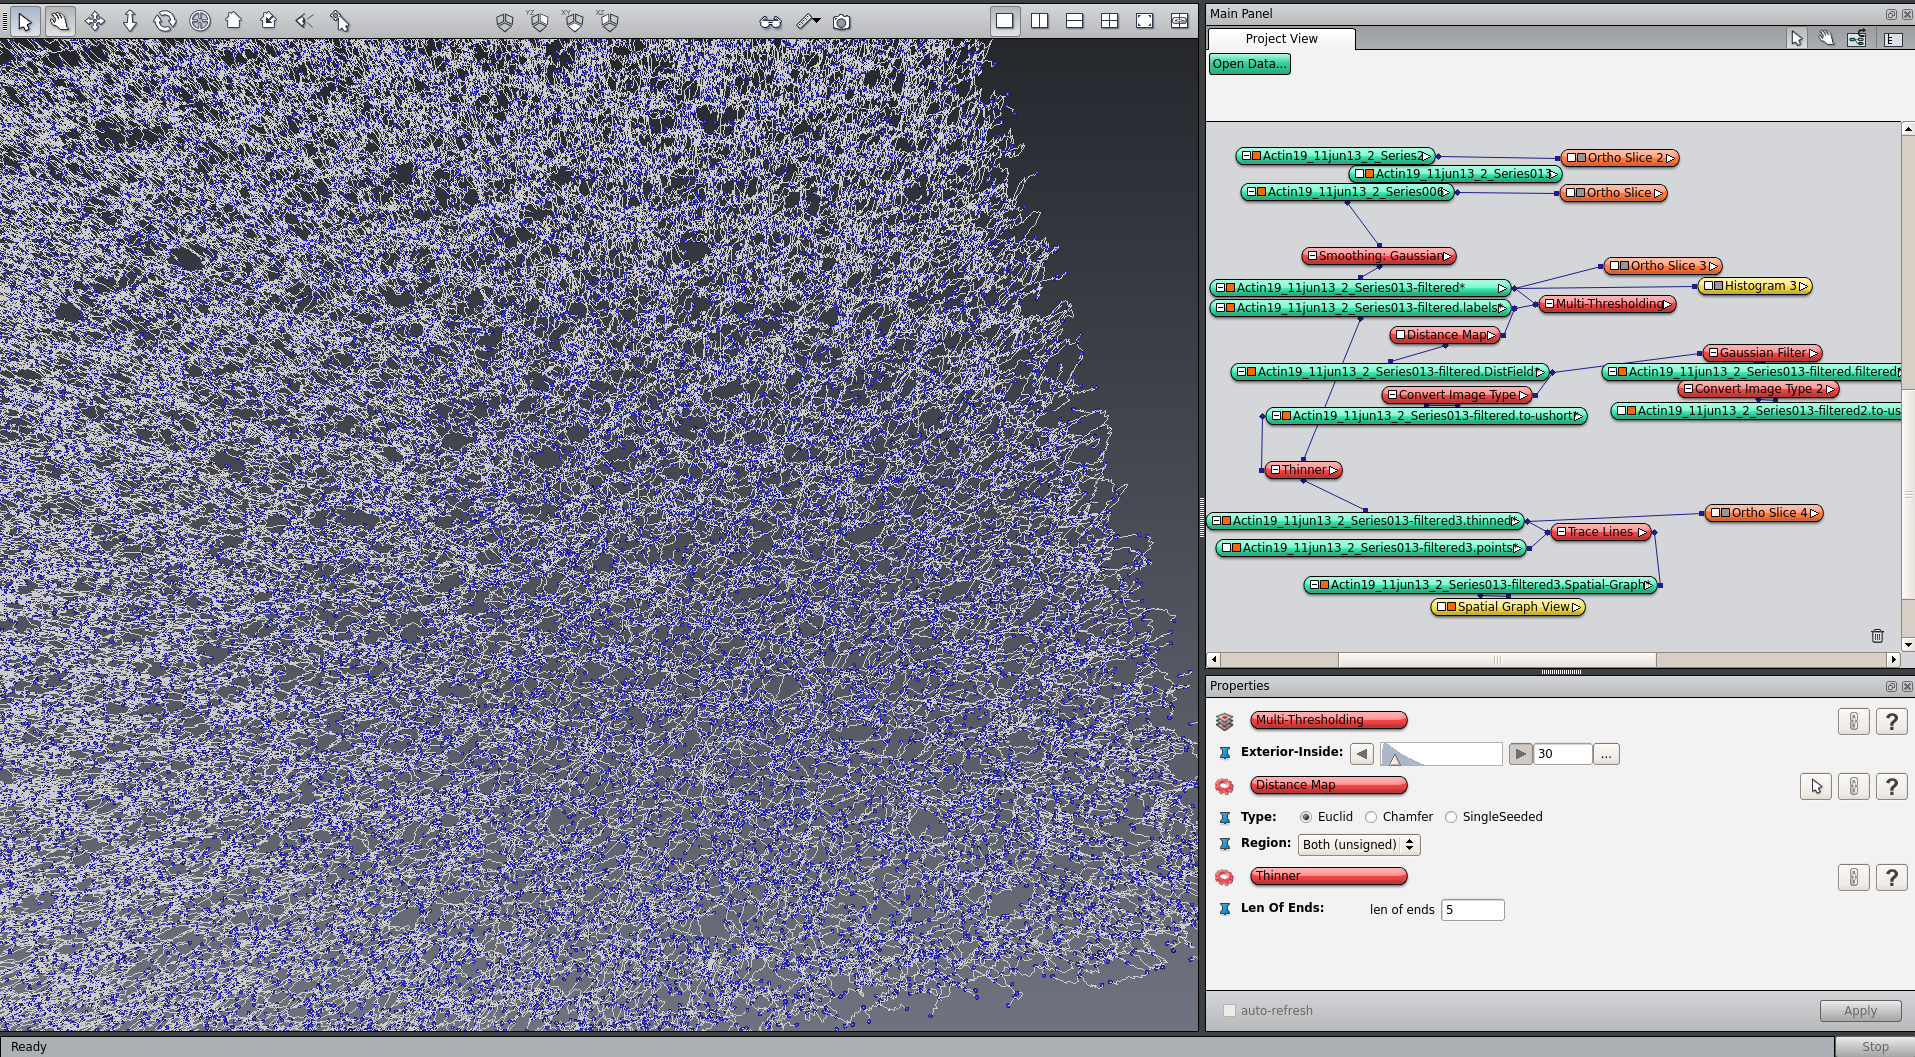
\includegraphics[width=0.9\textwidth]{Figures/chapter-image/avizo/workspace-wholedata.png}%

\caption[Avizo image: Actin network visualization and workspace]{Avizo
workspace. \emph{Left:} Visualization of the whole network of Actin data.
\emph{Top right:} Filters applied step by step. \emph{Bottom right:} Most
influential filters parameters, binarization threshold ($30$ in the image) and
skeletonization parameter: pruning of branches that length is lesser than the
threshold ($5$ in the image)}
\label{fig:avizo_workspace}
\end{figure}


\subsubsection{Avizo results:}
We have analyzed the whole stack of our confocal images of actin
($V=1024\times1024\times39$). The key parameters in Avizo are the binarization
$T$ and the pruning threshold $P$.

In Fig.\ref{fig:avizo_workspace}, a regular workspace in Avizo can be seen. The
different filters, the key parameters, and the result of the process, the actin
network are visualized.

In Fig.\ref{fig:avizo_histograms30} we have extracted statistical distributions
from the network that will be used in chapter \ref{Chapter-Reconstruction} for
the reconstruction of the network.

In Fig.\ref{fig:avizo_histograms21} we can check that statistical distributions
are quite robust versus small changes in the key parameters $T$ and $P$.

\begin{figure}[ht!]
  \centering
  \begin{subfigure}{0.32\textwidth}
    \centering
    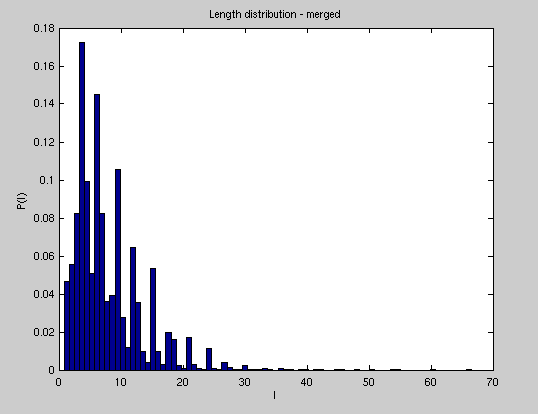
\includegraphics[width=0.92\textwidth]{Figures/chapter-image/avizo/ActinZ39b21l5-histo-length.png}%
    \label{avizo305-length}
  \end{subfigure}%
  \begin{subfigure}{0.32\textwidth}
    \centering
    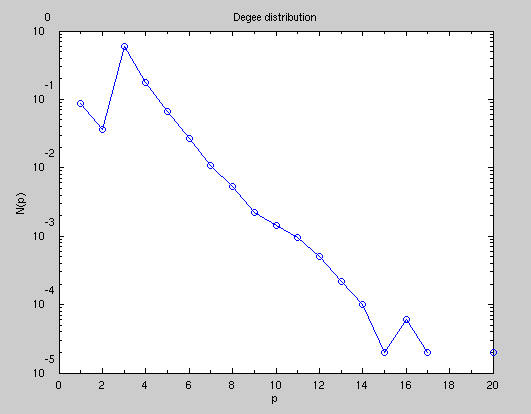
\includegraphics[width=0.92\textwidth]{Figures/chapter-image/avizo/ActinZ39b21l5-histo-degree.png}%
    \label{avizo305-degree}
  \end{subfigure}%
  \begin{subfigure}{0.32\textwidth}
    \centering
    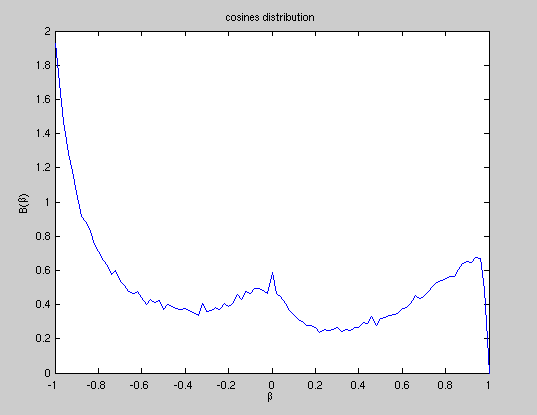
\includegraphics[width=0.92\textwidth]{Figures/chapter-image/avizo/ActinZ39b21l5-histo-cosines.png}
    \label{avizo305-cosines}
  \end{subfigure}

  \caption[Distributions of length, degree, and cosines with Avizo for
  actin with T=30,P=5]{Actin data analyzed with Avizo with binary threshold
    $T=30$ and pruning parameter $P=5$. \subref{avizo305-length} Length following a
    log-normal or exponential distribution. \subref{avizo305-degree} Degree
    following a geometrical distribution. \subref{avizo305-cosines}  Director
  cosines following an unknown distribution}
  \label{fig:avizo_histograms30}
\end{figure}

\begin{figure}[ht!]
  \centering
  \begin{minipage}{0.32\textwidth}
    \centering
    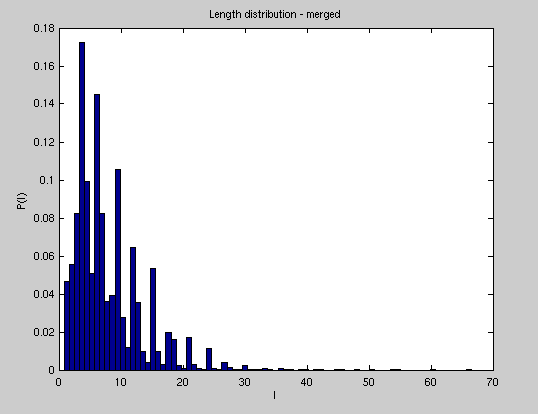
\includegraphics[width=0.92\textwidth]{Figures/chapter-image/avizo/ActinZ39b21l5-histo-length.png}%
  \end{minipage}
  \begin{minipage}{0.32\textwidth}
    \centering
    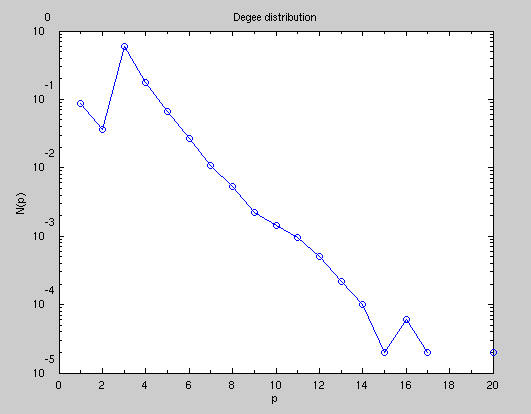
\includegraphics[width=0.92\textwidth]{Figures/chapter-image/avizo/ActinZ39b21l5-histo-degree.png}%
  \end{minipage}
  \begin{minipage}{0.32\textwidth}
    \centering
    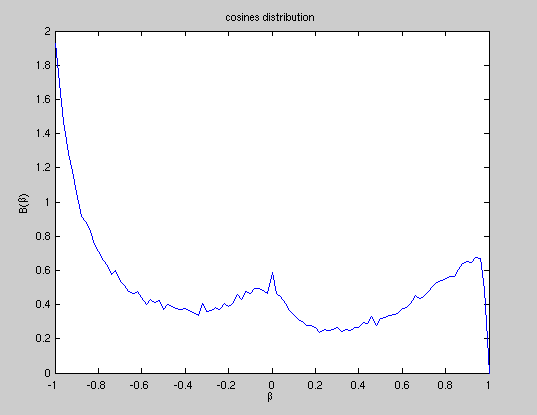
\includegraphics[width=0.92\textwidth]{Figures/chapter-image/avizo/ActinZ39b21l5-histo-cosines.png}%
  \end{minipage}
  \begin{minipage}{0.32\textwidth}
    \centering
    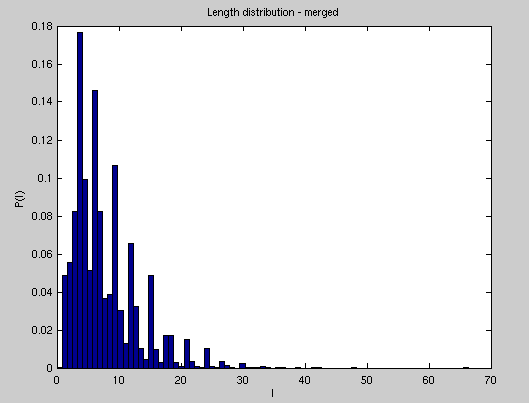
\includegraphics[width=0.92\textwidth]{Figures/chapter-image/avizo/ActinZ39b21l8-histo-length.png}%
  \end{minipage}
  \begin{minipage}{0.32\textwidth}
    \centering
    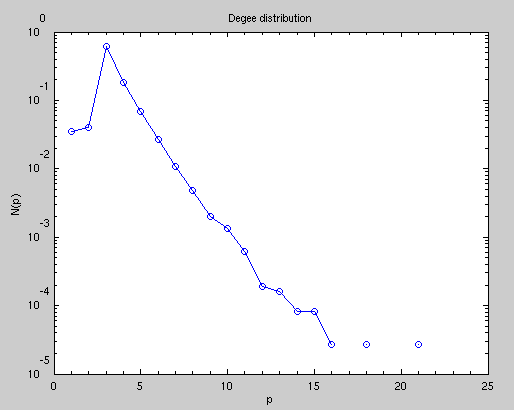
\includegraphics[width=0.92\textwidth]{Figures/chapter-image/avizo/ActinZ39b21l8-histo-degree.png}%
  \end{minipage}
  \begin{minipage}{0.32\textwidth}
    \centering
    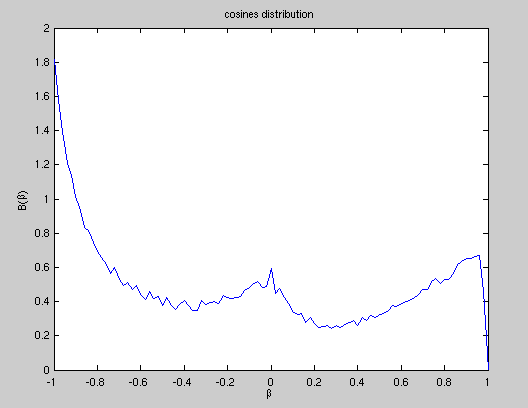
\includegraphics[width=0.92\textwidth]{Figures/chapter-image/avizo/ActinZ39b21l8-histo-cosines.png}%
  \end{minipage}

\caption[Distributions of length, degree, and cosines with Avizo for
actin with T=21,P=5]{Actin data analyzed with Avizo with binary threshold
$T=21$ and pruning parameter: $P=5$ in the first row, and  $P=8$ in the second
row. We can see that small changes in the parameters
does not affect much to the statistical distributions}
\label{fig:avizo_histograms21}
\end{figure}

The statistical distribution must be further compared with those in FIRE (with
a whole network), but we can see that the algorithm seems stable against minor
changes in the important parameters.

\section{Spatial Graph Extraction}%
\label{sec:spatial_graph_extraction}

From the skeletonization we get a thin image, where all the pixels belonging to an object in the binary image are reduced to a thin representation of it, in the sense that this generated skeleton is one-pixel wide.

From here, our task is to transform this thin image or skeleton into a \gls{graph}. A set of nodes connected to each other through edges. The first step, and also contributed to the DGtal library by the author is to get what we denominate a \textbf{raw graph}, a graph where each node is a voxel of the skeleton, and neighbor voxels have an edge connecting them.

For regular images, this raw graph is enormous, imagine a voxel in the interior of an object, this voxel will have 26 edges (degree = 26) connecting it to its surrounding nodes.
But for thin images, where the number of voxels is greatly reduced, this allow us to start using tools from graph theory to extract a more meaningful graph, a \gls{Spatial Graph}.

In a \gls{Spatial Graph} only nodes with degree different than 2 are considered vertices (see \autoref{fig:spatial_graph}). These end (degree = 1) and junction (degree > 2) nodes are connected to similar nodes via \glspl{Spatial Edge}, where the bending points (degree = 2) connecting those are stored in the spatial edge as \textbf{edge points} (see \autoref{fig:spatial_graph_intro_2} for an example). The rest of vertices are kept with the same connectivity as \glspl{Spatial Node}, adding its index or spatial position from the image.

This transform uses a Depth First Search (\gls{DFS}) visit, starting from end-points vertices (degree=1), it follows the connected neighbors (chain-nodes of degree 2) until it reaches another end-point or another vertex with degree 3 or more. When this happen, two \glspl{Spatial Node} are added to the new \gls{Spatial Graph} (the source where we started and the end node), and one \gls{Spatial Edge}, containing all the visited 2-degree pixels.

We keep visiting the raw graph with the \gls{DFS} algorithm, where the visited nodes are marked to avoid re-visiting them. We follow on with any non-visited junction nodes (degree > 2). And to finish, we search for any self-loops, circular structures where all nodes have degree 2. Because the graph doesn't allow self-loops, edges where source and target are the same node, we encode the self-loop into two nodes, the first is the original vertex, and the second one is created in the median of the \gls{Spatial Edge}. So these self loops are two nodes with two parallel edges of about the same number of edge-points between them.

The \gls{DFS} algorithms is quite fast thanks to its marking of already visited nodes. There are two filters that we can apply to the process that have an impact in the generated \gls{Spatial Graph}.

The original \textbf{Raw Graph} can be optionally post-processed, if there are three nodes with degree 3 connected between them, the longest edges (diagonals) are removed (see \autoref{subfig:graph_raw_merged}).

\begin{figure}[!htb]
  \centering
  \begin{subfigure}{0.5\textwidth}
    \centering
    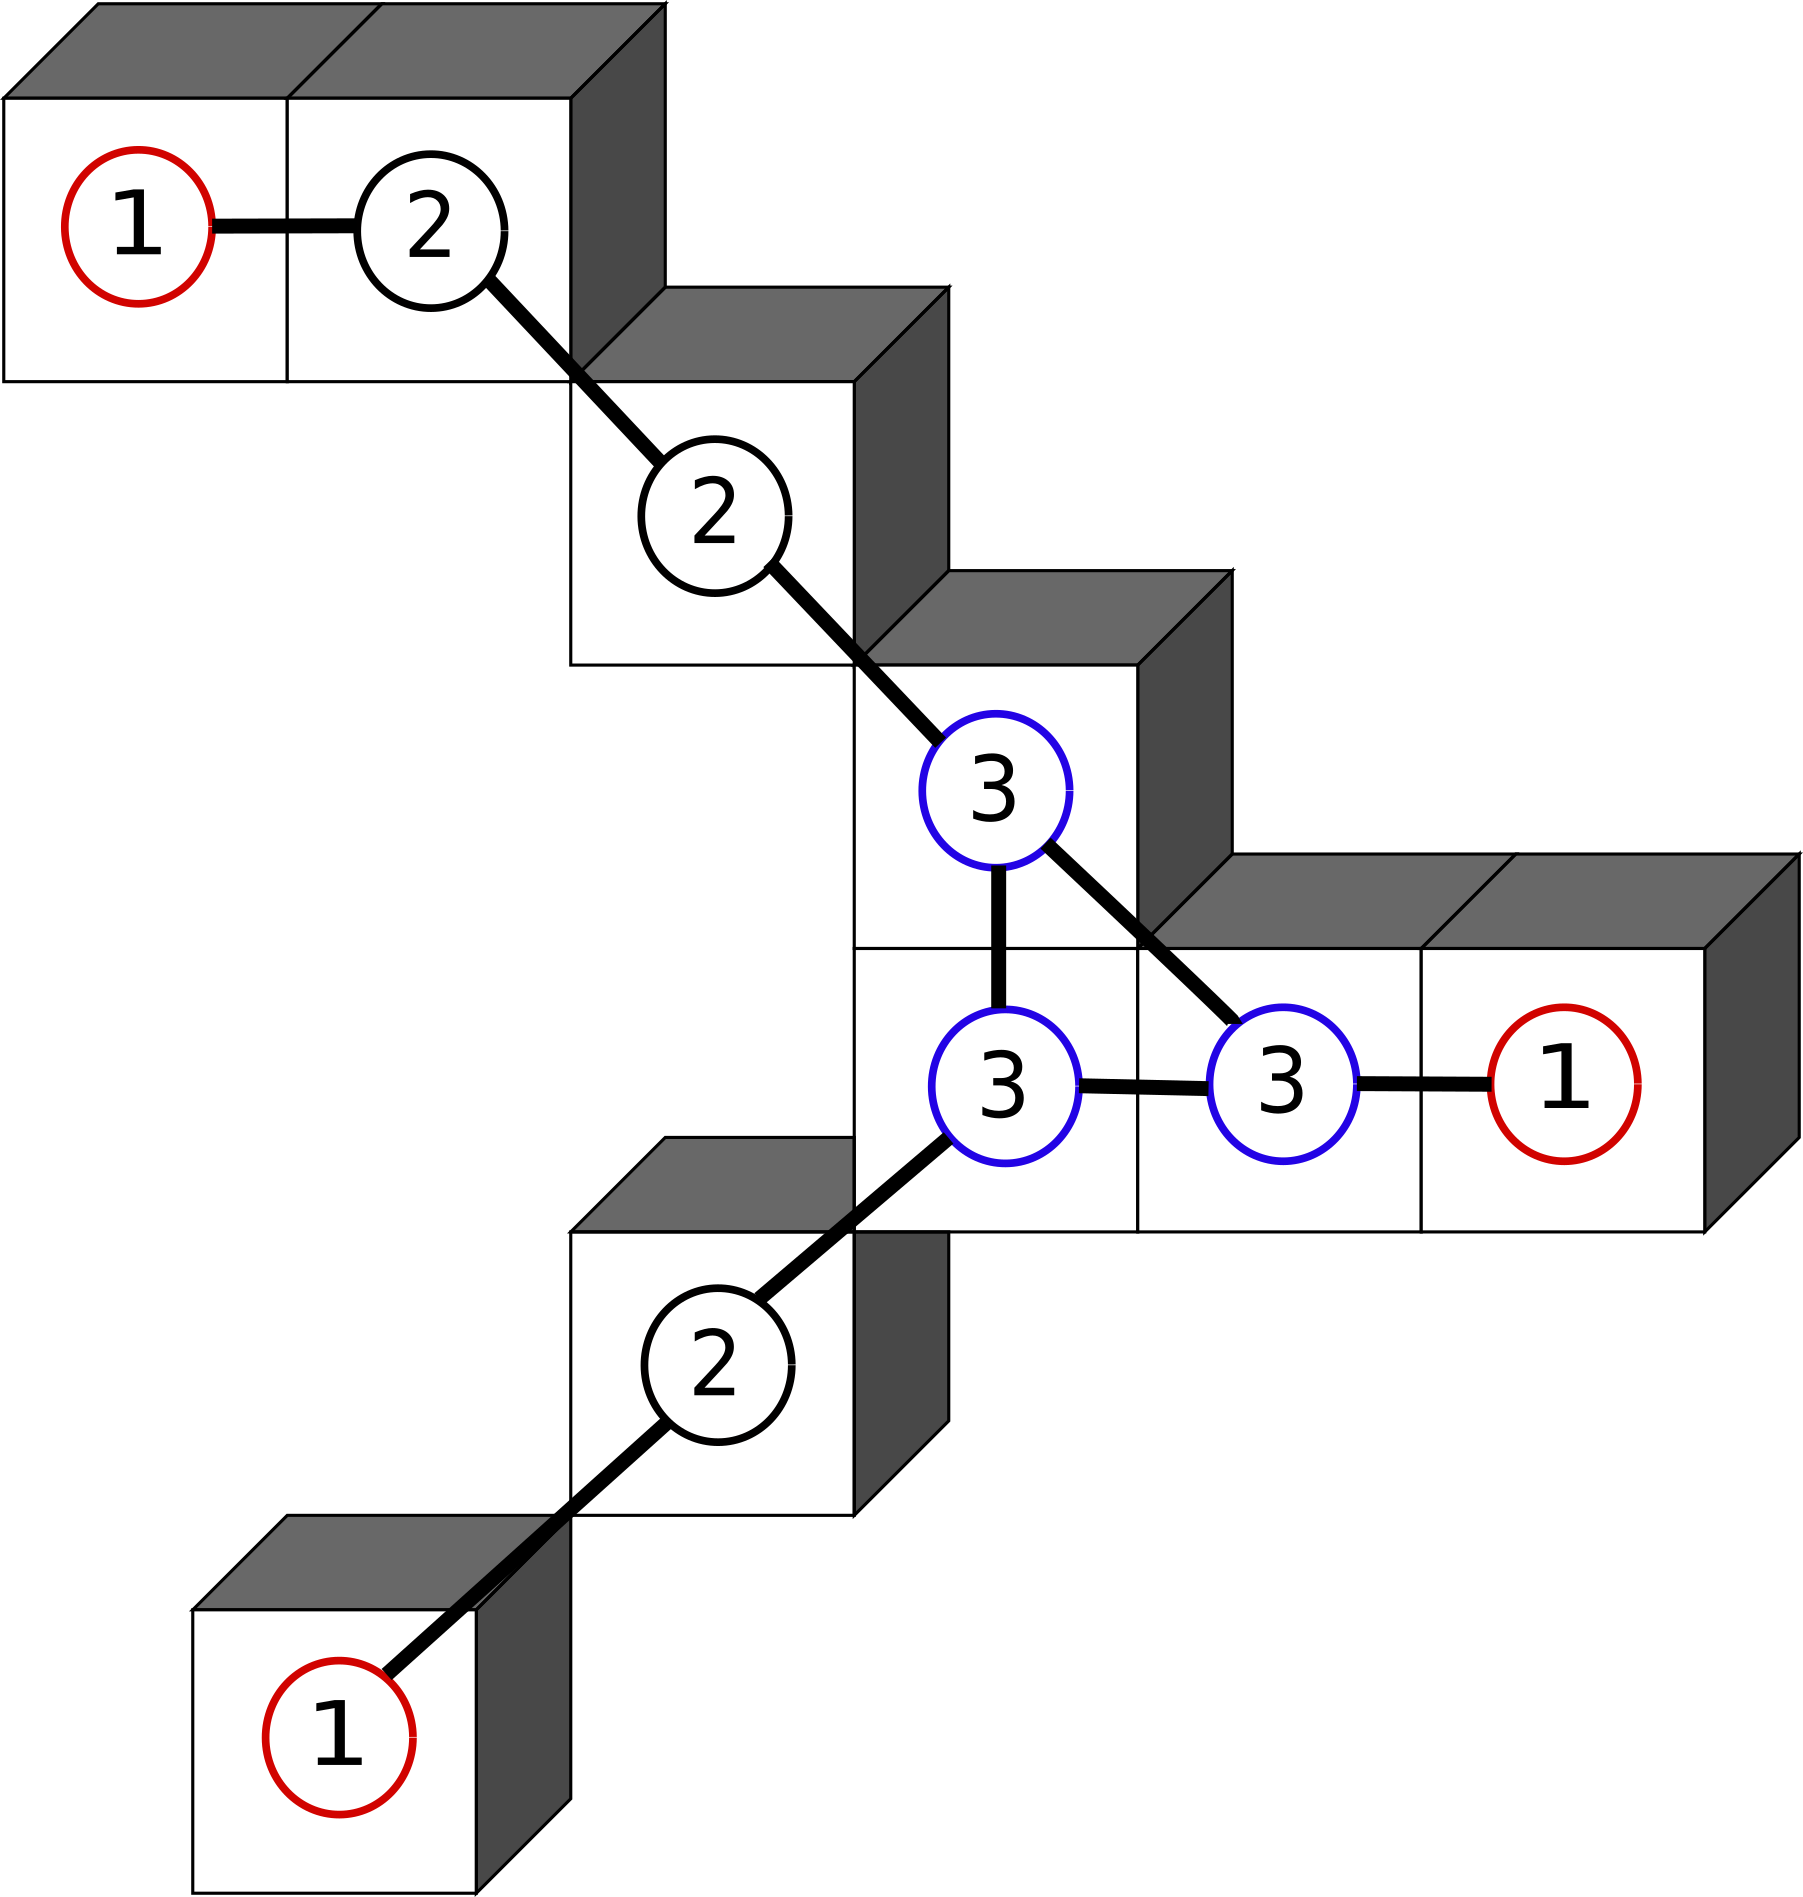
\includegraphics[width=0.9\textwidth]{Figures/chapter-image/dgtal/voxels_raw.png}%
    \caption{Raw Graph}
    \label{subfig:graph_raw}
  \end{subfigure}%
  \begin{subfigure}{0.5\textwidth}
    \centering
    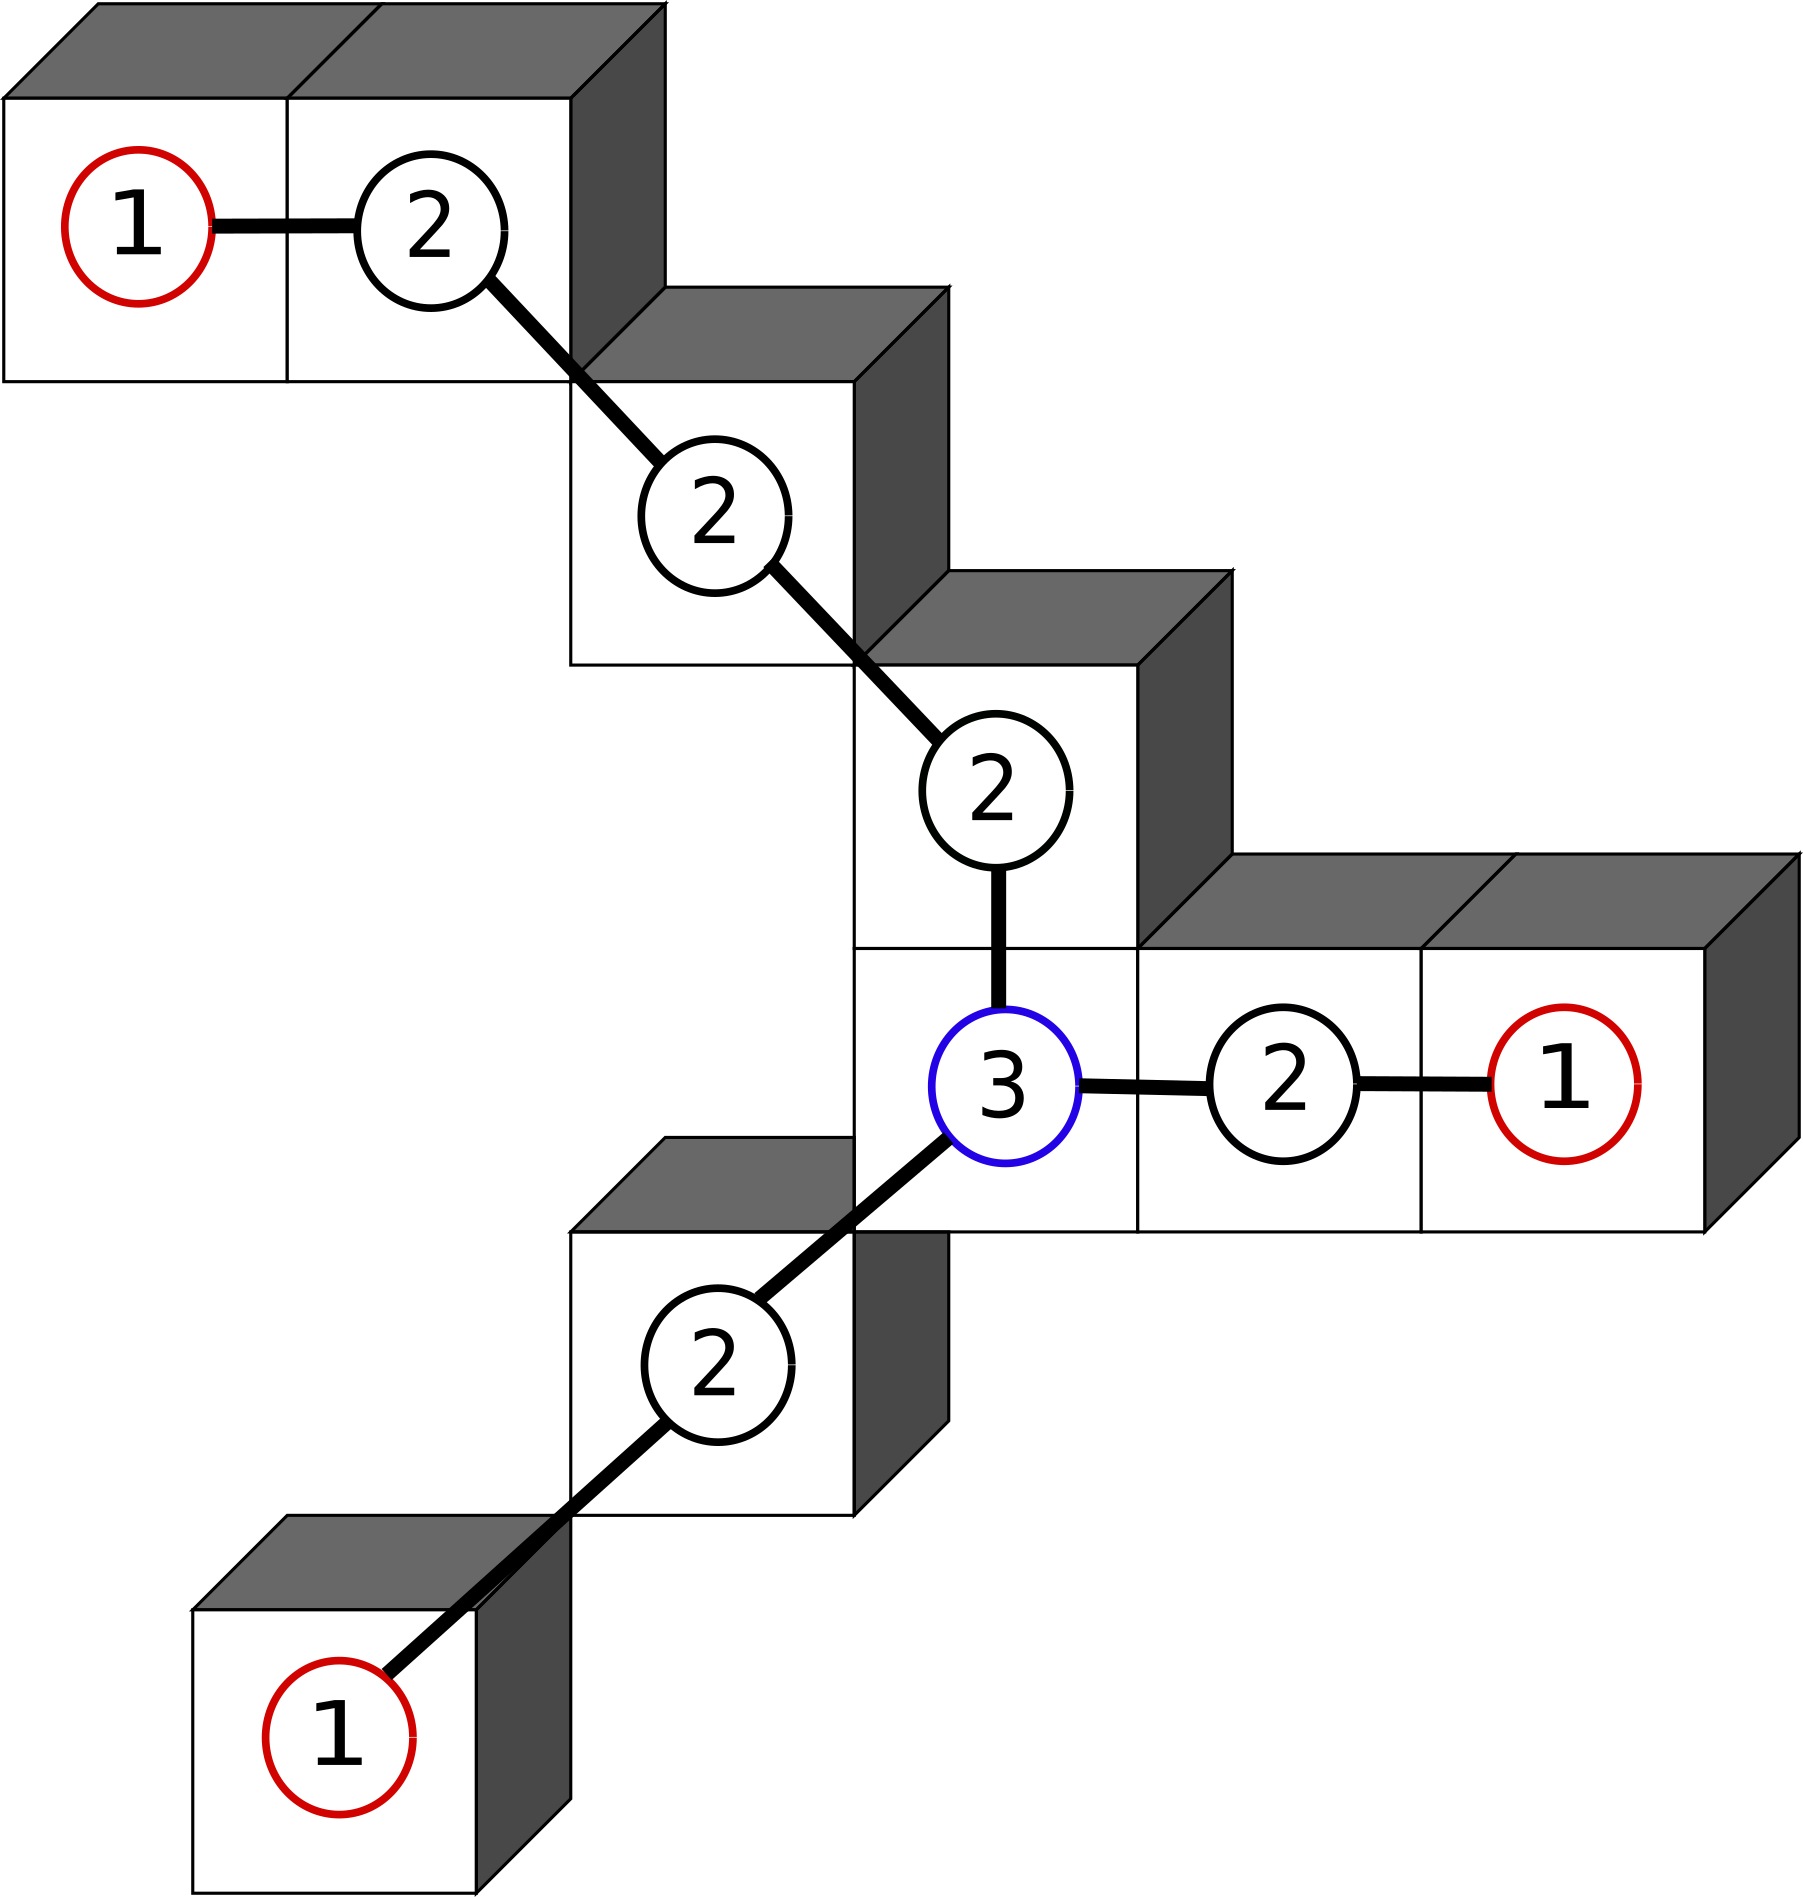
\includegraphics[width=0.9\textwidth]{Figures/chapter-image/dgtal/voxels_raw_merged.png}%
    \caption{Raw Graph merged}
    \label{subfig:graph_raw_merged}
  \end{subfigure}%
  \caption{Extracting the raw graph from the thin image and post processed to remove the largest edges between tri-connected nodes with degree 3. Numbers show the number of edges (degree) of each node. }
  \label{fig:raw_graph_extraction}
\end{figure}


\begin{figure}[!htb]
  \centering
  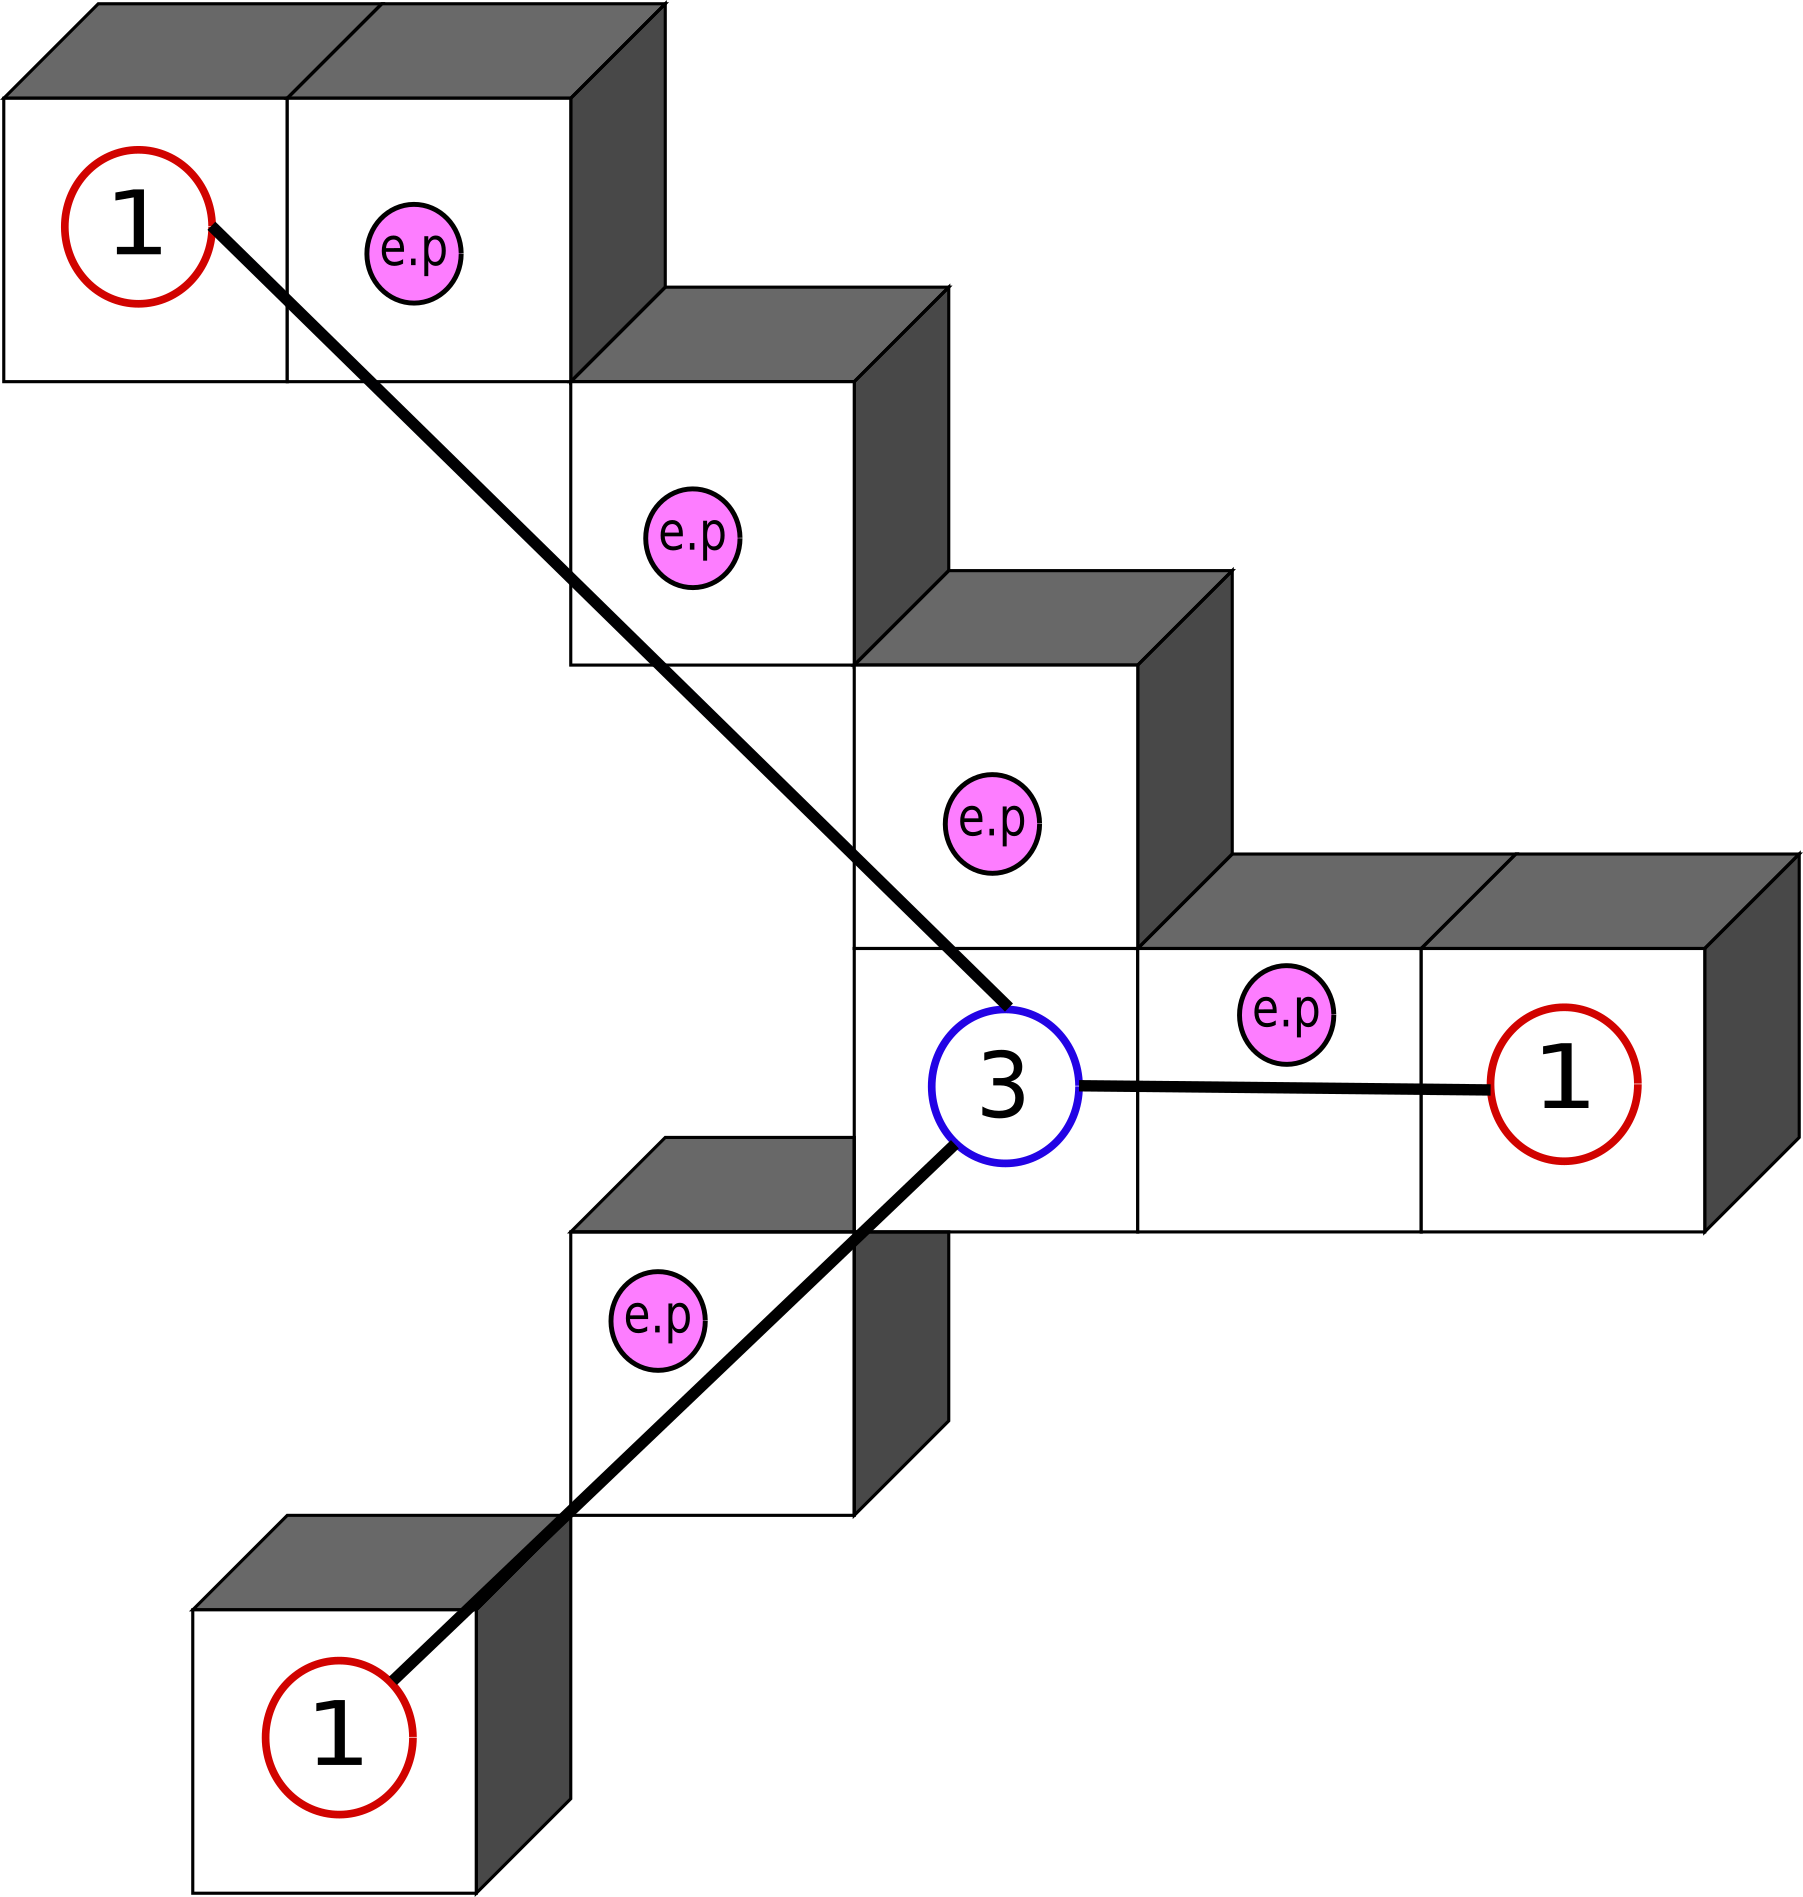
\includegraphics[width=0.45\textwidth]{Figures/chapter-image/dgtal/voxels_spatial_merge.png}%
  \caption{\gls{Spatial Graph} where vertices with degree 2 are deleted, and its position are stored as edge points in the new edges.}
  \label{fig:spatial_graph}
\end{figure}

The spatial graph give access to the complete network geometry, plus also allow us to analyze the architecture with sharper tools.

\section{Statistical distributions of graph properties}%
\label{sec:statistical_distributions_of_graph_properties}

With the spatial graph in hand we have at our disposal all the tool-box from the field of
complex networks to characterize the network plus all the geometrical measurements we might need due to the storage of positions of each node and edge points in the spatial graph.

Following Lindstrom approach to characterize networks from statistical distributions \cite{lindstrom_finite-strain_2013, lindstrom_biopolymer_2010}, we will compute the degree distribution, end-to-end distance between nodes (ignoring edge points), contour lengths between nodes (taking into account edge points), angles between adjacent edges and cosine directors of those angles.

The degree-distribution follows a geometric distribution, truncated for branch-points (only nodes with degree greater than 3) for all our networks, see \autoref{degree-dist}.

The end-to-end distance between nodes and the contour lengths distributions fits to a
log-normal distribution, see \autoref{length-dist}. This distribution is used to describe multiplicative processes in many fields,
in biology they are used to describe growth processes \cite{mitzenmacher_brief_2004}.

These distributions are the result of the generative processes in network formation, and can be used to infer the details of such processes and patterns \cite{frank_common_2009, frank_how_2014}.

The director cosines of the angles between adjacent edges is fitted to a truncated power series \cite{lindstrom_finite-strain_2013}, that fits well for all the networks studied, see \autoref{cosines-dist}.

\section{Results}%
\label{sec:sg_results}

We apply the described pipeline in previous sections to three set of volumetric images:

\begin{itemize}[topsep=0pt]
  \item \textbf{Actin: } Stack of images from Confocal Light Microscopy
  \item \textbf{Carrageenan: } Image from \gls{TEM} tomography
  \item \textbf{Pectin: } Image from \gls{TEM} tomography
\end{itemize}

\subsection{Actin}%
\label{sub:actin}
The actin network was prepared using 0.3 mg/ml actin in 40 mMol MgCl2 and stained with phalloidin.
The image was taken using Confocal Laser Scanning Microscopy (CLSM) with Leica Instrumentation (model TCS SP5).

The volumetric image used in this study has a size of 1024$\times$1024$\times$106 pixels, with resolution 0.505050745877353$\times$0.505050745877353$\times$1.00708103855232 \si{\micro\metre} per pixel.

The parameters used in the image pipeline:

\textbf{Denoise:}

\noindent Using the c++ script \citetitle*{phcerdan_rieszwaveletphaseanalysis_2018} \cite{phcerdan_rieszwaveletphaseanalysis_2018}.
\begin{minted}{bash}
export WAVELET_TYPE=Simoncelli # options: Held, Vow, Shannon
export LEVELS=4
export BANDS=4
rieszWaveletPhaseAnalysis -i ${INPUT_IMAGE} -o ${OUTPUT_FOLDER} \
       -w ${WAVELET_TYPE} -l ${LEVELS} -b ${BANDS}
\end{minted}

We apply an anisotropic denoise step with the itk filter CurvatureAnisotropicDiffusion,
using the python script  \citetitle*{phcerdan_denoise_input_2018} \cite{phcerdan_denoise_input_2018}.

\begin{minted}{bash}
export DENOISE_ITERATIONS=20
export DENOISE_CONDUCTANCE=2.0
export DENOISE_TIMESTEP=0.0625 #default optimal value for 3D
python denoise_input.py ${OUTPUT_WAVELET} ${OUTPUT_FOLDER} \
      ${DENOISE_ITERATIONS} ${DENOISE_CONDUCTANCE}
\end{minted}

Result: \autoref{fig:actin_denoised}.

\textbf{Segmentation:}
Apply a region growing algorithm as explained in \autoref{subsub:region_growing_segmentation},
using the c++ script  \citetitle*{phcerdan_regionGrowingSegmentation_2018} \cite{phcerdan_regionGrowingSegmentation_2018}.
\begin{minted}{bash}
export BIN_RG_LOWER=0.0
export BIN_RG_UPPER=5000
export BIN_SAFE_PERCENTAGE=0.2
regionGrowingSegmentation -i ${OUTPUT_DENOISE} -o ${OUTPUT_FOLDER}\
    -l ${BIN_RG_LOWER} -u ${BIN_RG_UPPER} -p ${BIN_SAFE_PERCENTAGE}
\end{minted}

And the hole filling algorithm described in \autoref{sub:hole_filling},
using the python script  \citetitle*{phcerdan_binary_denoise_3d_fillholes_iterative_2018} \cite{phcerdan_binary_denoise_3d_fillholes_iterative_2018}.

\begin{minted}{bash}
export HOLE_MAJORITY=3
export HOLE_RADIUS=1
export HOLE_ITERATIONS=10000
python binary_denoise_3d_fillholes_iterative.py ${OUTPUT_BINARY} ${OUTPUT_FOLDER}\
${HOLE_MAJORITY} ${HOLE_RADIUS} ${HOLE_ITERATIONS}
\end{minted}

Result: \autoref{fig:actin_segmentation}.

\textbf{Skeletonization}

Apply a thinning using the critical kernels framework contributed to DGtal (see \autoref{sub:critical_kernels_framework})
using the c++ script  \citetitle*{phcerdan_thin_2018} \cite{phcerdan_thin_2018}.

\begin{minted}{bash}
export SKEL_SELECT=dmax
export SKEL_TYPE=1isthmus
export SKEL_PERSISTENCE=2
thin --input ${OUTPUT_SEGMENTATION} -o ${OUTPUT_FOLDER} \
  --select ${SKEL_SELECT} --skel ${SKEL_TYPE} \
  -p ${PERSISTENCE} --foreground white
\end{minted}

The option \textit{dmax} generates a distance map as shown in \autoref{subfig:actin_dmap}.

Result: \autoref{subfig:actin_skeleton}.

\textbf{Spatial Graph Extraction}

The conversion from the thin image to the spatial graph representation as described in \autoref{sec:spatial_graph_extraction},
uses the c++ script  \citetitle*{phcerdan_analyze_graph_2018} \cite{phcerdan_analyze_graph_2018}.

\begin{minted}{bash}
export GRAPH_IGNORE_SHORT_EDGES=1
export GRAPH_SPACING="5.05050745877353E-07 5.05050745877353E-07 1.00708103855232E-06"
analyze_graph --input ${OUTPUT_SKELETONIZATION} \
 --exportReducedGraph ${OUTPUT_FOLDER} --exportData ${GRAPH_DATA_FOLDER}
 --reduceGraph --removeExtraEdges  --mergeThreeConnectedEdges \
 --ignoreAngleBetweenParallelEdges \
 --ignoreEdgesShorterThan ${GRAPH_IGNORE_SHORT_EDGES} \
 --spacing ${GRAPH_SPACING}
\end{minted}

\textit{exportData} compute the graph properties: degree, end-to-end distances, contour lengths, angle and cosine directors, and save them into a file.

\textit{exportReducedGraph} outputs the spatial graph in a .dot (graphviz) format, similar to \autoref{fig:spatial_graph_intro_2}, that be read by any graph library.

\textit{removeExtraEdges} applies the removal of diagonal edges at intersection, as described in \autoref{subfig:graph_raw_merged}.

The result is a spatial graph, \autoref{fig:actin_graph} shows a representation of that graph without representing contour lengths, lines are just straight lines connecting end-to-end nodes. Node glyphs are not represented to avoid cluttering the 3D scene.


% \begin{minted}{bash}
% # Wavelet Phase Analysis
% export WAVELET_TYPE=Simoncelli
% export LEVELS=4
% export BANDS=4
% # Anisotropic Denoise
% export DENOISE_ITERATIONS=20
% export DENOISE_CONDUCTANCE=2.0
% export DENOISE_TIMESTEP=0.0625
% ## Region Growing Binarization
% export BIN_RG_LOWER=0.0
% export BIN_RG_UPPER=5000
% export BIN_SAFE_PERCENTAGE=0.2
% ## Hole Filling
% export HOLE_MAJORITY=3
% export HOLE_RADIUS=1
% export HOLE_ITERATIONS=10000
% ## Skeletonization
% export SKEL_SELECT=dmax
% export SKEL_TYPE=1isthmus
% export SKEL_PERSISTENCE=2
% ## Spatial Graph Extraction
% export GRAPH_IGNORE_SHORT_EDGES=1
% export GRAPH_SPACING=""
% \end{minted}


% \begin{figure}[!htb]
\begin{figure}[H]
  \centering
  \begin{subfigure}{0.33\textwidth}
    \centering
    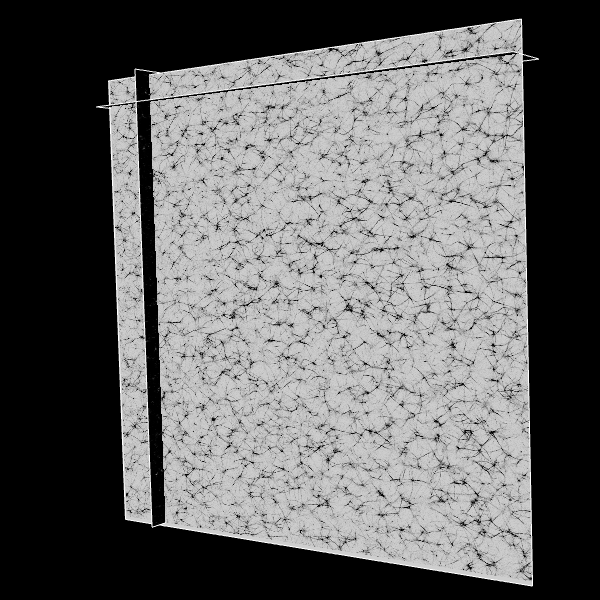
\includegraphics[width=0.9\linewidth]{Figures/chapter-image/pipeline_screenshots/actin_volume.png}
    \caption{Original volume}
    \label{fig:actin_original}
  \end{subfigure}%
  \begin{subfigure}{0.33\textwidth}
    \centering
    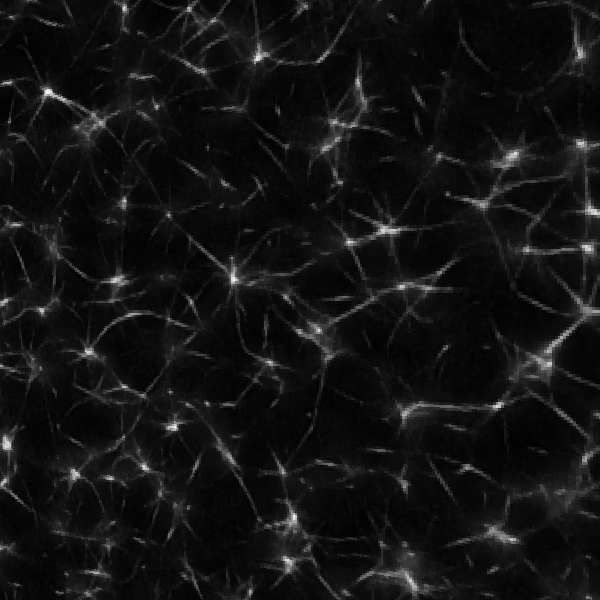
\includegraphics[width=0.9\linewidth]{Figures/chapter-image/pipeline_screenshots/actin_denoised_wavelet_anisotropic.png}
    \caption{Denoised.}
    \label{fig:actin_denoised}
  \end{subfigure}%
  \begin{subfigure}{0.33\textwidth}
    \centering
    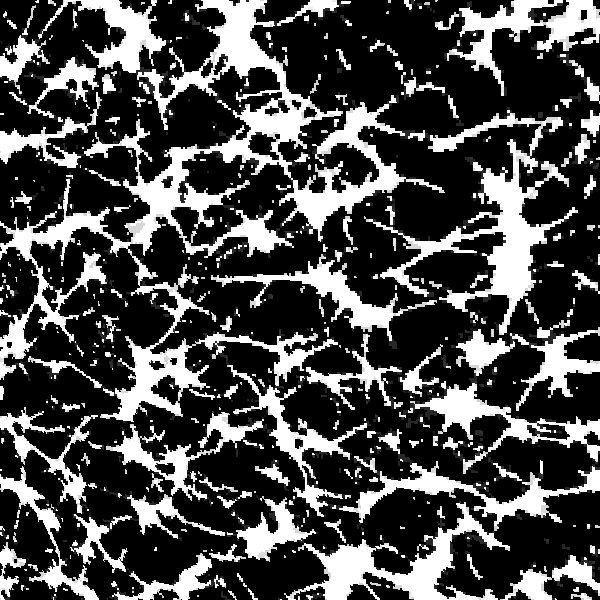
\includegraphics[width=0.9\linewidth]{Figures/chapter-image/pipeline_screenshots/actin_segmented_sparse.png}
    \caption{Segmentation.}
    \label{fig:actin_segmentation}
  \end{subfigure}\\[1ex]
  \begin{subfigure}{0.33\textwidth}
    \centering
    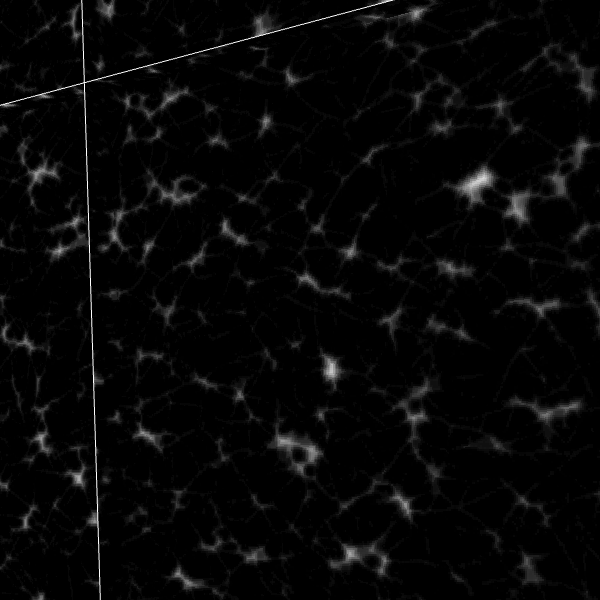
\includegraphics[width=0.9\linewidth]{Figures/chapter-image/pipeline_screenshots/actin_dmap.png}
    \caption{Distance Map}
    \label{subfig:actin_dmap}
  \end{subfigure}%
  \begin{subfigure}{0.33\textwidth}
    \centering
    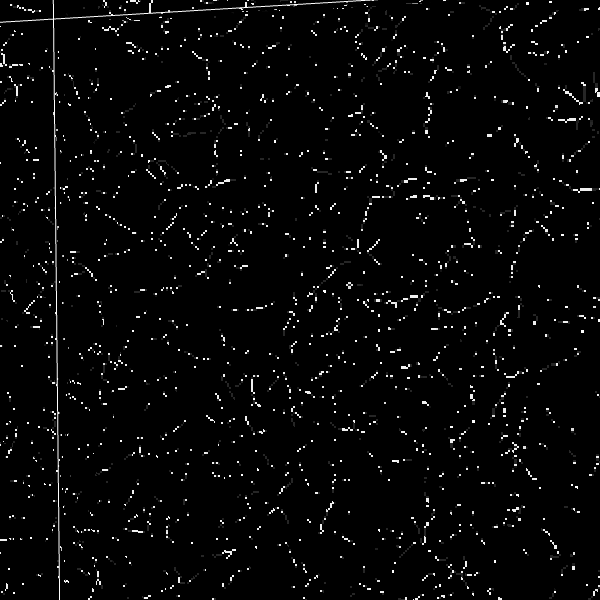
\includegraphics[width=0.9\linewidth]{Figures/chapter-image/pipeline_screenshots/actin_skeleton.png}
    \caption{Skeletonization (p = 2).}
    \label{subfig:actin_skeleton}
  \end{subfigure}%
  \begin{subfigure}{0.33\textwidth}
    \centering
    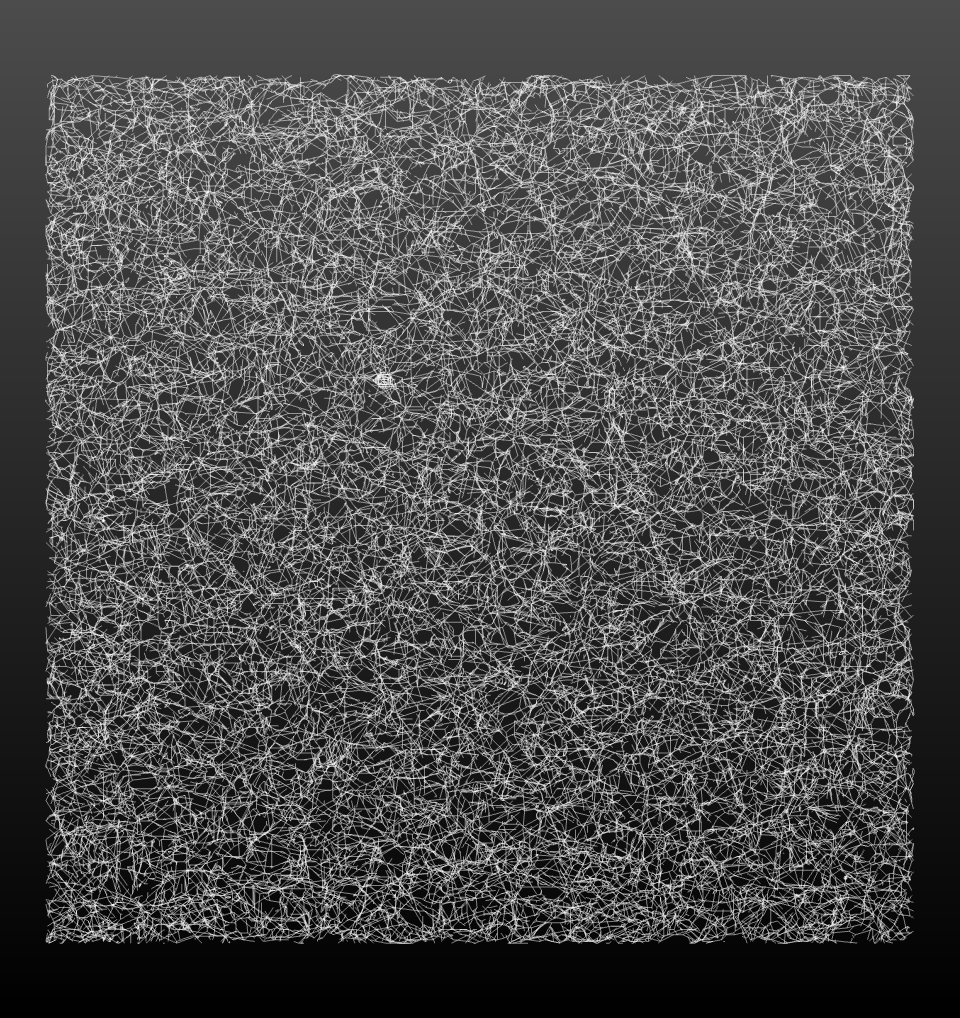
\includegraphics[width=0.9\linewidth]{Figures/chapter-image/pipeline_screenshots/actin_graph.png}
    \caption{Graph}
    \label{fig:actin_graph}
  \end{subfigure}%
  \caption{Actin spatial graph extraction steps.}
  \label{fig:actin_all}
\end{figure}

\textbf{Fit graph data to distributions}

We fit the graph data generated in the analysis to statistical distributions depending on the property, as described in \autoref{sec:statistical_distributions_of_graph_properties}.
An estimation of the $R^2$ of the fit using Effron's formula \cite{lindstrom_finite-strain_2013} is shown.
The degree is fitted the mentioned truncated geometric distribution also showing the percentage of end-nodes, see \autoref{subfig:actin_degree}.

It uses the python script  \citetitle*{phcerdan_fit_to_distribution_from_data_2018} \cite{phcerdan_fit_to_distribution_from_data_2018} with parameters:

\begin{minted}{bash}
export HISTO_ETE_BINS=30
export HISTO_COSINES_BINS=21
export HISTO_CONTOUR_BINS=30
python fit_to_distributions_from_data ${GRAPH_DATA} \
   ${HISTO_ETE_BINS} ${HISTO_COSINES_BINS} ${HISTO_CONTOUR_BINS} log
\end{minted}

\begin{figure}[H]
% \begin{figure}[!htb]
  \centering
  \begin{subfigure}{0.5\textwidth}
    \centering
    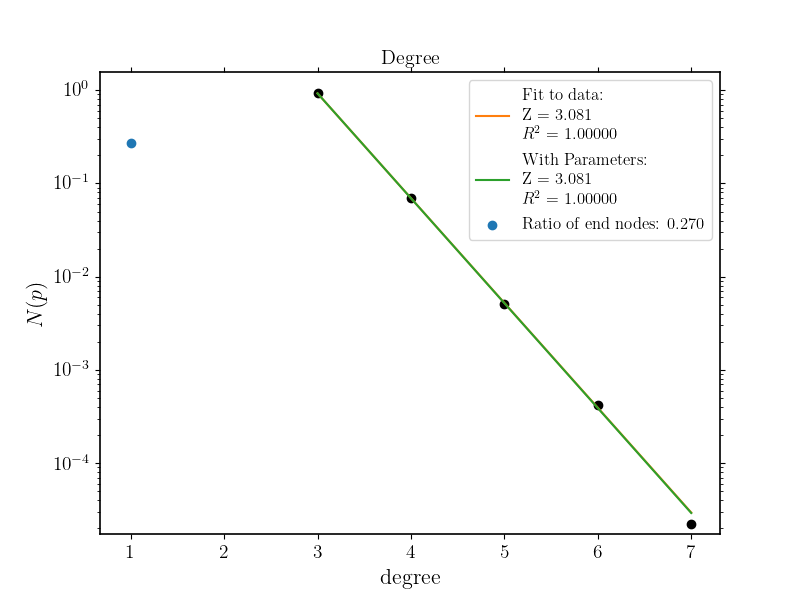
\includegraphics[width=0.99\linewidth]{Figures/chapter-image/pipeline_screenshots/actin_degree_tile4_c_m.png}
    \caption{Degree distribution. Geometric}
    \label{subfig:actin_degree}
  \end{subfigure}%
  \begin{subfigure}{0.5\textwidth}
    \centering
    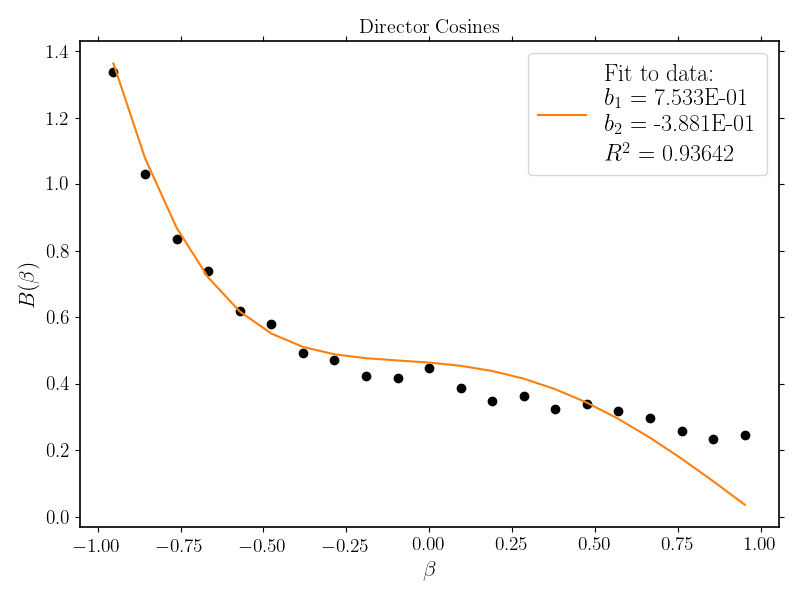
\includegraphics[width=0.99\linewidth]{Figures/chapter-image/pipeline_screenshots/actin_cosines_tile4_c_m_iPA_iShort1_bins21.png}
    \caption{Director cosines. Truncated (3) power-series.}
    \label{subfig:actin_cosines}
  \end{subfigure}\\[1ex]
  \begin{subfigure}{0.5\textwidth}
    \centering
    \includegraphics[width=0.99\linewidth]{Figures/chapter-image/pipeline_screenshots/actin_ete_distance_tile4_c_m_iPA_iShort1_bins30.png}
    \caption{End-to-End node distances. Log-normal}
    \label{subfig:actin_ete}
  \end{subfigure}%
  \begin{subfigure}{0.5\textwidth}
    \centering
  \includegraphics[width=0.99\linewidth]{Figures/chapter-image/pipeline_screenshots/actin_contour_length_tile4_c_m_iPA_iShort1_bins30.png}
    \caption{Contour lengths. Log-normal}
    \label{subfig:actin_contour}
  \end{subfigure}
  \caption{Statistical distributions (PDF) of actin network.}
  \label{fig:actin_thin}
\end{figure}

\subsection{TEM preparation}%
\label{sub:tem_preparation}

The polysaccharides carrageenan and pectin are imaged with \gls{TEM} tomography with the preparation published in \citep{hernandez-cerdan_structural_2018-2} and reproduced here for completion:

Gels were fixed with 0.1\% Ruthenium Red and phosphate buffered 2.5\% glutaraldehyde prior to dehydration in a graded ethanol series and embedding in an epoxy resin (ProCure 812, ProSciTech, Thuringowa, Australia). Fixation mechanisms for aldehydes are known to some extent from protein crystallographic studies, where in particular covalent bonding with lysine residues is employed \cite{wine_elucidation_2007}, but no comparable studies exist for polysaccharides. We found that Ruthenium Red was essential for maintaining sample integrity during dehydration. We observed that this was due to the formation of a skin on the gel pieces. The role of glutaraldehyde in preserving or altering structure is unknown but our observations suggest that there is no effect on the bulk structure down to the level of individual molecules, where some combination of fixation and staining changes the native morphology. Indeed, some deviation from native structure must be expected due to the use of one or more of these reagents. Sections with nominal thickness of 150 nm were cut with an ultramicrotome and post-stained with 2\% uranyl acetate prior to visualisation. Previous work using tomography to acquire images from pecin gels in 3D \cite{mansel_zooming_2015} suggests that this post-staining is effective throughout the section thickness. Imaging areas were pre-irradiated for 15 minutes at low magnification prior to image acquisition. Two-dimensional micrographs were recorded on a JEOL JEM-1400 transmission electron microscope with a $\text{LaB}_6$ cathode operated at 120 kV under low-dose conditions with synchronised beam blanking and acquisition.

\subsection{Carrageenan}%
\label{sub:carrageenan}


Ion-exchanged sodium carrageenan samples were provided by Dupont. Relevant salt solutions (30 mM KCl  or 300 mM NaCl) were first made by dissolving the required amount of salt in a volumetric flask and using millQ water. The required amount of dry carrageenan in order to produce 1\% w/w solutions was then weighed out and subsequently suspended in the relevant salt solution. The solutions were then heated to \SI{60}{\degreeCelsius} while stirring until all powder was dissolved. This solution was then loaded hot into the requisite sample cells for \gls{TEM}.

The volumetric tomography image used in this study has a size of 896$\times$896$\times$64 pixels, with resolution 0.86$\times$0.86$\times$0.86 \nm per pixel.

\textbf{Denoise:}

We use total variation denoising in these particular TEM images using the python script \citetitle*{phcerdan_denoise_tv_2018} \cite{phcerdan_denoise_tv_2018}, which uses proxTV library \cite{barbero_modular_2014}.

\begin{minted}{bash}
export TV_LAMBDA=20
python denoise_tv ${INPUT_IMAGE} ${OUTPUT_FOLDER} ${TV_LAMBDA}
\end{minted}

Result: \autoref{fig:carra_denoised}.

The rest of the pipeline is the same than for actin \autoref{sub:actin}, changing BIN\_SAFE\_PERCENTAGE, and GRAPH\_SPACING, including the fit to distributons

\begin{minted}{bash}
## Region Growing Binarization
export BIN_RG_LOWER=0.0
export BIN_RG_UPPER=5000
export BIN_SAFE_PERCENTAGE=0.05
## Hole Filling
export HOLE_MAJORITY=3
export HOLE_RADIUS=1
export HOLE_ITERATIONS=10000
## Skeletonization
export SKEL_SELECT=dmax
export SKEL_TYPE=1isthmus
export SKEL_PERSISTENCE=2
## Spatial Graph Extraction
export GRAPH_IGNORE_SHORT_EDGES=1
export GRAPH_SPACING="0.86E-09 0.86E-09 0.86E-09"
## Fit graph data to distributions
export HISTO_ETE_BINS=30
export HISTO_COSINES_BINS=21
export HISTO_CONTOUR_BINS=30
\end{minted}

\begin{figure}[H]
% \begin{figure}[!htb]
  \centering
  \begin{subfigure}{0.33\textwidth}
    \centering
    \includegraphics[width=0.9\linewidth]{Figures/chapter-image/pipeline_screenshots/carra_original_tile1.png}
    \caption{Original volume}
    \label{fig:carra_original}
  \end{subfigure}%
  \begin{subfigure}{0.33\textwidth}
    \centering
    \includegraphics[width=0.9\linewidth]{Figures/chapter-image/pipeline_screenshots/carra_denoised_tv20_tile1.png}
    \caption{Denoised.}
    \label{fig:carra_denoised}
  \end{subfigure}%
  \begin{subfigure}{0.33\textwidth}
    \centering
    \includegraphics[width=0.9\linewidth]{Figures/chapter-image/pipeline_screenshots/carra_segmented_tile1.png}
    \caption{Segmentation.}
    \label{fig:carra_segmentation}
  \end{subfigure}\\[1ex]
  \begin{subfigure}{0.33\textwidth}
    \centering
    \includegraphics[width=0.9\linewidth]{Figures/chapter-image/pipeline_screenshots/carra_dmap_tile1.png}
    \caption{Distance Map}
    \label{subfig:carra_dmap}
  \end{subfigure}%
  \begin{subfigure}{0.33\textwidth}
    \centering
    \includegraphics[width=0.9\linewidth]{Figures/chapter-image/pipeline_screenshots/carra_skeleton_tile1.png}
    \caption{Skeletonization (p = 2).}
    \label{subfig:carra_skeleton}
  \end{subfigure}%
  \begin{subfigure}{0.33\textwidth}
    \centering
    \includegraphics[width=0.9\linewidth]{Figures/chapter-image/pipeline_screenshots/carra_graph_tile1.png}
    \caption{Graph}
    \label{fig:carra_graph}
  \end{subfigure}%
  \caption{Carrageenan spatial graph extraction steps.}
  \label{fig:carra_all}
\end{figure}

\begin{figure}[H]
% \begin{figure}[!htb]
  \centering
  \begin{subfigure}{0.5\textwidth}
    \centering
    \includegraphics[width=0.99\linewidth]{Figures/chapter-image/pipeline_screenshots/carra_degree_tile1_c_m.png}
    \caption{Degree distribution. Geometric}
    \label{subfig:carra_degree}
  \end{subfigure}%
  \begin{subfigure}{0.5\textwidth}
    \centering
    \includegraphics[width=0.99\linewidth]{Figures/chapter-image/pipeline_screenshots/carra_cosines_tile1_c_m_iPA_iShort1_bins21.png}
    \caption{Director cosines. Truncated (3) power-series.}
    \label{subfig:carra_cosines}
  \end{subfigure}\\[1ex]
  \begin{subfigure}{0.5\textwidth}
    \centering
    \includegraphics[width=0.99\linewidth]{Figures/chapter-image/pipeline_screenshots/carra_ete_distance_tile1_c_m_iPA_iShort1_bins30.png}
    \caption{End-to-End node distances. Log-normal}
    \label{subfig:carra_ete}
  \end{subfigure}%
  \begin{subfigure}{0.5\textwidth}
    \centering
    \includegraphics[width=0.99\linewidth]{Figures/chapter-image/pipeline_screenshots/carra_contour_length_tile1_c_m_iPA_iShort1_bins30.png}
    \caption{Contour lengths. Log-normal}
    \label{subfig:carra_contour}
  \end{subfigure}
  \caption{Statistical distributions (PDF) of Carrageenan K network.}
  \label{fig:carra_thin}
\end{figure}

\subsection{Pectin}%
\label{sub:Pectin}

The gelation method exploited herein has been described in detail previously \cite{mansel_zooming_2015} and used in \cite{hernandez-cerdan_structural_2018-2}.
To summarize: a commercially available pectin sample that had a high degree of methylesterification (DM) (78\%) was modified using a processive pectin methyl esterase (PME) extracted from oranges and sourced from Sigma, to obtain a block-wise sample with DM of around 40\%, and the resulting polymer freeze dried. The polymeric fine structure was measured using capillary electrophoresis as described elsewhere. Subsequently a solution was made by dissolving \SI{0.02}{\g} of the freeze-dried pectin in \SI{1.5}{\ml} of deionized water. Next \SI{0.16}{\g} of glucono delta-lactone (GDL) was dissolved in water and mixed with the pectin solution as quickly as possible, in order to minimize any hydrolysis of GDL occurring before mixing, while being careful not to form bubbles. This solution was then loaded into the requisite sample cells for \gls{TEM}.

The volumetric tomography image used in this study has a size of 1000$\times$1000$\times$32 pixels, with resolution 1.72$\times$1.72$\times$1.72 \nm per pixel.

The pipeline is the same than for carragenan \autoref{sub:carrageenan}, with the exception of GRAPH\_SPACING
\begin{minted}{bash}
# TV denoising
export TV_LAMBDA=20
## Region Growing Binarization
export BIN_RG_LOWER=0.0
export BIN_RG_UPPER=5000
export BIN_SAFE_PERCENTAGE=0.05
## Hole Filling
export HOLE_MAJORITY=3
export HOLE_RADIUS=1
export HOLE_ITERATIONS=10000
## Skeletonization
export SKEL_SELECT=dmax
export SKEL_TYPE=1isthmus
export SKEL_PERSISTENCE=2
## Spatial Graph Extraction
export GRAPH_IGNORE_SHORT_EDGES=1
export GRAPH_SPACING="1.72E-09 1.72E-09 1.72E-09"
## Fit graph data to distributions
export HISTO_ETE_BINS=30
export HISTO_COSINES_BINS=21
export HISTO_CONTOUR_BINS=30
\end{minted}

\begin{figure}[H]
% \begin{figure}[!htb]
  \centering
  \begin{subfigure}{0.33\textwidth}
    \centering
    \includegraphics[width=0.9\linewidth]{Figures/chapter-image/pipeline_screenshots/pectin_original.png}
    \caption{Original volume}
    \label{fig:pectin_original}
  \end{subfigure}%
  \begin{subfigure}{0.33\textwidth}
    \centering
    \includegraphics[width=0.9\linewidth]{Figures/chapter-image/pipeline_screenshots/pectin_denoised_tv20.png}
    \caption{Denoised.}
    \label{fig:pectin_denoised}
  \end{subfigure}%
  \begin{subfigure}{0.33\textwidth}
    \centering
    \includegraphics[width=0.9\linewidth]{Figures/chapter-image/pipeline_screenshots/pectin_segmented.png}
    \caption{Segmentation.}
    \label{fig:pectin_segmentation}
  \end{subfigure}\\[1ex]
  \begin{subfigure}{0.33\textwidth}
    \centering
    \includegraphics[width=0.9\linewidth]{Figures/chapter-image/pipeline_screenshots/pectin_dmap.png}
    \caption{Distance Map}
    \label{subfig:pectin_dmap}
  \end{subfigure}%
  \begin{subfigure}{0.33\textwidth}
    \centering
    \includegraphics[width=0.9\linewidth]{Figures/chapter-image/pipeline_screenshots/pectin_skeleton.png}
    \caption{Skeletonization (p = 2).}
    \label{subfig:pectin_skeleton}
  \end{subfigure}%
  \begin{subfigure}{0.33\textwidth}
    \centering
    \includegraphics[width=0.9\linewidth]{Figures/chapter-image/pipeline_screenshots/pectin_graph.png}
    \caption{Graph}
    \label{fig:pectin_graph}
  \end{subfigure}%
  \caption{Pectin spatial graph extraction steps.}
  \label{fig:pectin_all}
\end{figure}

\begin{figure}[H]
% \begin{figure}[!htb]
  \centering
  \begin{subfigure}{0.5\textwidth}
    \centering
    \includegraphics[width=0.99\linewidth]{Figures/chapter-image/pipeline_screenshots/pectin_degree_c_m.png}
    \caption{Degree distribution. Geometric}
    \label{subfig:pectin_degree}
  \end{subfigure}%
  \begin{subfigure}{0.5\textwidth}
    \centering
    \includegraphics[width=0.99\linewidth]{Figures/chapter-image/pipeline_screenshots/pectin_cosines_c_m_iPA_iShort1_bins21.png}
    \caption{Director cosines. Truncated (3) power-series.}
    \label{subfig:pectin_cosines}
  \end{subfigure}\\[1ex]
  \begin{subfigure}{0.5\textwidth}
    \centering
    \includegraphics[width=0.99\linewidth]{Figures/chapter-image/pipeline_screenshots/pectin_ete_distance_c_m_iPA_iShort1_bins30.png}
    \caption{End-to-End node distances. Log-normal}
    \label{subfig:pectin_ete}
  \end{subfigure}%
  \begin{subfigure}{0.5\textwidth}
    \centering
    \includegraphics[width=0.99\linewidth]{Figures/chapter-image/pipeline_screenshots/pectin_contour_length_c_m_iPA_iShort1_bins30.png}
    \caption{Contour lengths. Log-normal}
    \label{subfig:pectin_contour}
  \end{subfigure}
  \caption{Statistical distributions (PDF) of Pectin network.}
  \label{fig:pectin_thin}
\end{figure}

\section{Conclusions}%
\label{sec:conclusions_image}

We were able to generate an image pipeline to extract the network architecture
of biopolymers of different scale, proteins and polysaccharides.
The network architecture is represented as a \gls{Spatial Graph}, containing the connectivity and
the geometric information to fully describe the network geometry.

Computing some graph properties, degree, end-to-end distances, contour lengths and cosine directors of angles of the different biopolymers, we see that they share the same statistical distribution for those properties. These distributions were reported already for collagen and fibrin networks \cite{lindstrom_finite-strain_2013}, but never in polysaccharides. We think this universality in distributions, which suggests independence from the scale of the polymer, originates from the network formation with cross-links.

The spatial graph can be used by theoreticians as a starting scaffold for dynamic simulations, instead of the over-simplified methods currently used in literature (see \autoref{sec:network_structure} for a survey). This might help for models able to predict the whole range of dynamics in non-affine networks, micro-networks behaviours, and it is able to integrate cross-links dynamics.

All the code is freely available and open to be re-used, modified and improved by interested users, with the only condition that any modification to the source code must be open, for all of us enjoy the improvements.



% The comparison between the FIRE algorithm in Matlab and Avizo is not trivial.
% Here I select the most important:
%
% {\large\textbf{FIRE algorithm in Matlab}}
% \begin{itemize}
% \item \textbf{Pros:}
%
% \begin{itemize}
%   \item \textbf{Open source code.} With the free access to the code I have the
%   opportunity to change and manipulate all the process in function of my needs.
%   This process is also quite instructive. 
%
%   \item \textbf{Reliable.} This method has been tested carefully
% \citep{stein_mathematical_2007}, and its reliability has been demonstrated in fluorescence confocal
% images of stiff collagen filaments.
% \end{itemize}
% \item  \textbf{Contras:}
% \begin{itemize}
%   \item \textbf{No beautiful visualization.} I can implement a code to visualize
%   the network in $3D$, but it is not as detailed as in Avizo
%   \item \textbf{Slow.} It is not implemented using parallel capabilities, and
%   can be quite slow for large networks.
% \end{itemize}
% \end{itemize}
%
% {\large\textbf{Avizo}}
% \begin{itemize}
%   \item \textbf{Pros:}
%
%
% \begin{itemize}
%   \item \textbf{$3D$ filters.} All the filters, and image manipulation
%   algorithms comes from the computer vision community and they work in $2D$.
%   There are reliable open source libraries(tested code) of $2D$ filters, but
%   not in $3D$.
%   The implementation of a $3D$ from a $2D$ isn't usually that hard, but it is
%   extra work that Avizo solves for you, with the drawback of having no access to
%   those libraries because its condition of commercial software.
%    \item \textbf{Visualization of the network.} It uses a computer graphics
%    library called VTK (open source) to visualize the network in a beautiful and
%    effective way.
%    \item \textbf{Skeletonization.} It uses a skeletonization method based on the
%    distance map that seems fast and effective. But knowing the exact algorithm
%    would be helpful.
% \end{itemize}
% \item \textbf{Contras:}
% \begin{itemize}
%   \item \textbf{Commercial Software.} It is really expensive, we have access to
%   it thanks to a collaboration agreement with Fonterra researchers. 
%   \item \textbf{Black Box.} It
%   shares the drawbacks of commercial software: it is impossible to
%   manipulate it at your will to fit your requirements. Having no access to the
%   algorithms is like using a black box, you don't know exactly what is
%   happening behind the curtains. 
%   \item \textbf{Development Toolbox.} There is a development add-on (extra
%   cost), where you can create new filters and interact with the rest of the framework
%   in Avizo. I have to carefully study if the efforts of learning this tool will
%   have a decisive improvement in the image analysis.
% \end{itemize}
% \end{itemize}
% FIBER algorithm seems very reliable, but I think it has
% room for at least, technical improvement, such as parallel implementation.
% The way it expands nucleation points using traces along the maximal ridges
% of the distance map doesn't seem to be based in any well
% established/optimized skeletonization algorithm from the computer vision
% community. The free access to the code allow us to improve it or change it at our will.
%
% The main drawback of Avizo is that I cannot access or alter the
% skeletonization algorithm.
% To solve that, I should implement my own skeletonization algorithm, using the
% latest computer vision techniques\citep{bai_skeleton_2007}, and then interact with Avizo to represent the network.
% The TEM microscopy analysis
% requirements will be the key input to decide the way to follow.
%
% Despite the algorithm used, we have to choose the set of parameters that best reproduces the topology (i.e.
% architecture) of the network at the end of the image analysis process.
% I cite \citet{stein_algorithm_2008}: ``We have found that with confocal
% images of fluorescently labeled collagen, it is relatively straight forward
% to chose a threshold that qualitatively appears to maintain
% network topology". I agree with that affirmation but if it holds with
% other materials, or other microscopy techniques (TEM) have to be tested. The
% unique way to test it is to rely on the best image analyser that we have available, our brain.
%
% To generate a network filtered by the brain, we follow the chains, count
% the nodes, and draw a small volume of the network, using as unique analyzer our vision, and then
% compare it with the topology of the automatized algorithm
% \citep{chandran_affine_2006}.
% Despite the suggested complexity of the process,
% it is straight forward to choose, at least, a short range of threshold values that approximates the architecture. The
%  information extracted from the image analysis process seems to be quite robust
% against the fine-tuning of the parameters, sharing the same shape with the
% changes.
% These distributions, especially the angle, differ along
% different materials, as shown in the literature
% \citep{lindstrom_finite-strain_2013}, and also comparing actin data from our lab
% with collagen data from the literature\citep{lindstrom_biopolymer_2010}. These
% differences create a good opportunity to relate them with mechanical properties of the bulk
% system, in the context of non-affine networks.
%

